\documentclass[11pt]{article}
\usepackage[margin=1.1in]{geometry}
\usepackage{booktabs}
\usepackage{amsmath}
\usepackage{amssymb}
\usepackage{graphicx}
\usepackage[hidelinks]{hyperref}
\usepackage{xcolor}
\usepackage{authblk}
\usepackage{tikz}
\usetikzlibrary{arrows.meta}
\usepackage[ruled]{algorithm2e}
\usepackage[backend=biber,style=numeric,sorting=none]{biblatex}
\addbibresource{refs.bib}
\newcommand{\map}{\mathop{\bigoplus}\limits}
\newcommand{\txtop}[1]{\mathop{\mathtt{#1}}\limits}

% a table header cell on two lines: \stackhead[r]{loss\\recovered}
\newcommand{\stackhead}[2][l]{\begin{tabular}[b]{@{}#1@{}}#2\end{tabular}}

\newcommand{\expr}{\txtop{expression}}

\newcommand{\fn}{\txtop{function}}
\newcommand{\linear}{\txtop{linear}}
\newcommand{\relu}{\txtop{ReLU}}
\newcommand{\topk}{\txtop{TopK}}
\newcommand{\sigmoid}{\txtop{sigmoid}}
\newcommand{\tanhl}{\txtop{tanh}}
\newcommand{\softmax}{\txtop{softmax}}
\newcommand{\argmin}{\txtop{argmin}}
\newcommand{\argmax}{\txtop{argmax}}
\newcommand{\einsum}{\txtop{einsum}}
\newcommand{\colsum}{\txtop{colsum}}

\newcommand{\encoder}{\txtop{encoder}}
\newcommand{\decoder}{\txtop{decoder}}
\newcommand{\classifier}{\txtop{classifier}}
\newcommand{\partitioner}{\txtop{dict}}

\newcommand{\bilinearblock}{\txtop{BilinearBlock}}
\newcommand{\dictblock}{\txtop{DictBlock}}
\newcommand{\dictenc}{\txtop{DictEnc}}
\newcommand{\ontologizer}{\txtop{Ontologizer}}

\SetKwProg{Fn}{Function}{}{end}
\SetKwProg{Dat}{Data}{}{end}

\SetKwInOut{Hyper}{Hyperparameters}

\SetKwFunction{softmax}{softmax}
\SetKwFunction{MSE}{MSE}
\SetKwFunction{L1}{L1}
\SetKwFunction{transpose}{transpose}
\SetKwFunction{matmul}{matmul}
\SetKwFunction{dist}{dist}
\SetKwFunction{eucl}{euclidean}
\SetKwFunction{cossim}{cossim}
\SetKwFunction{sindiff}{sindiff}
\SetKwFunction{pca}{pca}
\SetKwFunction{knn}{knn}

\SetKwFunction{sample}{sample}
\SetKwFunction{loss}{loss}
\SetKwFunction{train}{train}

\SetKwFunction{Type}{Type}
\SetKwFunction{List}{List}
\SetKwFunction{Arch}{Arch}
\SetKwFunction{Params}{Params}
\SetKwFunction{Model}{Model}

\SetKwFunction{Linear}{Linear}
\SetKwFunction{Bilinear}{Bilinear}
\SetKwFunction{NLinear}{NLinear}
\SetKwFunction{NLinearBlock}{NLinearBlock}
\SetKwFunction{DictBlock}{DictBlock}
\SetKwFunction{DictEnc}{DictEnc}
\SetKwFunction{Ontologizer}{Ontologizer}
\SetKwFunction{SAE}{SAE}

\newcommand{\todo}[1]{\textcolor{red}{[TODO: #1]}}
\newcommand{\fvu}{\mathrm{FVU}_w}

\title{Dictionary Learning as Unsupervised Steering-Vector Generation:\\
Ontologizers vs.\ Sparse Autoencoders on SONAR Sentence Embeddings}
\author[1]{Keira Wiechecki}
\author[1]{Jade Zaslavsky}

\affil[1]{Wakaru Labs \\
	\texttt{kaw504@nyu.edu}}
\date{\today --- working notes, results preliminary}

\begin{document}
\maketitle

\begin{abstract}
The Ontologizer is a multihead, multilayer dictionary-learning
architecture whose design goal is \emph{unsupervised steering-vector
generation}: a stack of competitive classifier ``heads'' reconstructing an
embedding space should discover the space's natural contrastive clusters,
MoEfying the representation into small, nameable classification tasks
whose within-head entry swaps are steering moves. We evaluate two forms of
it --- the softmax (soft-code) Ontologizer and a straight-through
(hard-code) arm whose forward pass \emph{is} the argmax --- against
field-standard top-$k$ sparse autoencoders (SAEs) trained on identical
cached SONAR multilingual sentence embeddings under an identical whitened
reconstruction objective. The battery covers a reconstruction-vs-capacity
Pareto, categorical-form and semantic-coherence tests of head structure,
cross-model feature splitting and seed stability, downstream text
fidelity through the paired M2M100 decoder, language probing, shrinkage,
steering fidelity in text and embedding space, and blinded
auto-interpretability; a \emph{structural-ablation ladder} of SAE variants
attributes effects to specific structure. Preliminary findings:
(i) for soft codes, contrast-set structure is expensive in reconstruction
--- the plain-SAE frontier dominates the Ontologizer's deviation code at
every capacity; (ii) trained soft heads are contrast sets --- within-head
decode directions \emph{repel} (96\% of heads below a random-group null);
(iii) categorical form exists precisely when trained in as hard selection;
(iv) per-latent lenses --- $k$-sparse probing, per-feature detection ---
mis-measure classifier codes, and detection F1 is largely a measure of
code density; (v) a single-layer grouped-softmax SAE reproduces the
reference Ontologizer's structure and text fidelity. (vi) The
straight-through arm makes the discrete code the model: its argmax and
soft rows agree to four decimals where the softmax model's differ by nine
orders of magnitude, and at 1900 index bits and no continuous
coefficients it reaches $\fvu$ $0.154$ against $0.261$ for an SAE spending
625 coefficients --- after an initialization fix worth a third of its
error. (vii) At matched bits, parameters and code utilization the residual
cascade is worth $1.79\times$ over a flat layer, and the measured source
is the pairing between each stage's input and the sample's own earlier
error; the same cascade makes single-head interventions leak into
$\sim$60\% of other heads. (viii) Two seeds reach identical error while no
individual head --- partition, contribution, subspace or Gram ---
reproduces above a same-shape null, so head-level claims currently lack a
foundation. (ix) No head is a language variable in any arm; the strongest
head is a topic/genre head. (x) Non-negativity forces a collinear
dictionary at a third of the signed effective rank for $2.4\%$ of $\fvu$.
\end{abstract}

\section{Evaluation frame}

The comparisons below were largely built on SAE-native terms ---
per-feature monosemanticity, sparse probing, reconstruction at matched
sparsity --- and we report them unchanged. But the Ontologizer's goal is
not a monosemantic dictionary. It is an \emph{unsupervised generator of
steering vectors}: each head is a $k$-way classifier over its input,
trained only by reconstruction pressure, and the hope is that a series of
such classifiers finds the most natural contrastive clusters in the
embedding space. Interpretability value is then expected from
\emph{MoEfication}: decomposing the space into small classification tasks
--- one per head --- each nameable in isolation, with within-head entry
swaps as the steering primitive (forcing head $h$ from its argmax entry to
entry $k'$ moves the decode along exactly the dimension head $h$
classifies).

Under this frame the evaluation questions are: (a)~what does contrast-set
structure cost in reconstruction (the Pareto and ladder); (b)~do trained
heads actually behave as contrastive classifiers (categorical form,
semantic anti-coherence); (c)~are the learned tasks \emph{natural} ---
nameable, stable across runs, aligned with generative factors of the data
(seed reproducibility, language and topic alignment); and (d)~is the
steering primitive good --- consistent effect, low collateral, at least
matching supervised diff-of-means vectors and SAE decoder-row addition
(steering fidelity). Metrics that ask whether \emph{individual latents}
are concept-aligned remain informative about the SAE side but are the
wrong lens for classifier codes, and we flag them as such where they
appear.

Question (c) has a prerequisite that the original battery took for
granted: a head can only be named if it is the same head on every run.
Section~\ref{sec:seeds} tests that directly and finds it does not hold,
which conditions every per-head result in this document.

\section{Related work}

No single line of prior work covers this combination; each commitment has
a nearest neighbour.

\paragraph{Discrete and routed dictionaries.}
A \texttt{DictBlock} head --- a softmax over $k$ entries, summed across
heads --- is soft product quantization~\cite{jegou2011}, and the residual
layer stack is soft residual VQ, the codec lineage of
SoundStream~\cite{zeghidour2021}; that literature treats codes as
compression and does not read codebooks as features. The straight-through
arm (Section~\ref{sec:ste}) makes the analogy literal: with an argmax
forward and a softmax surrogate gradient~\cite{bengio2013} it is a
residual product quantizer with non-negative atoms. Codebook
Features~\cite{tamkin2023} is the closest interpretability ancestor (VQ
bottlenecks finetuned into a network, hidden state a sum of a few
discrete codes), but its codes are read per-code, not as classifiers, and
there is no intervention grammar over within-codebook swaps. Switch
SAEs~\cite{mudide2025} route activations among expert SAEs purely as a
compute optimization; notably their experts collapse into redundant
ensembles that duplicate features --- exactly the failure mode
\texttt{headstruct.py}/\texttt{headcoh.py} instrument, and the opposite of
what trained heads show here (within-head directions repel).
MoEfication~\cite{zhang2022} supplies the frame's name but decomposes
already-trained MLPs post hoc; here the partition is the training
objective's own discovery.

\paragraph{Structured SAEs.}
The field's main structure axis is nesting by scale: Matryoshka
SAEs~\cite{bussmann2025} train nested dictionaries to curb feature
absorption~\cite{chanin2025}, and Tree SAE~\cite{cao2026} learns explicit
hierarchies. Rung 3 (\texttt{k32\_p5}) imports exactly the matryoshka
commitment into the ladder; the Ontologizer's axis is instead
\emph{partition into exhaustive, mutually exclusive heads}. Both lines ask
whether an architectural commitment buys interpretability that code
density alone does not explain --- the auto-interp results below answer
``not per-latent describability,'' while the description-coherence view is
where the partition begins to pay.

\paragraph{Embedding-space substrate.}
SAEs over dense text embeddings became a subfield in 2025--2026:
discretizing retrieval embeddings~\cite{park2025decodingdenseembeddingssparse}, data-analysis
toolkits~\cite{jiang2026interpretableembeddingssparseautoencoders},
human-concept alignment~\cite{shin2026aligningsentenceembeddingshuman}. All
are single-layer top-$k$ SAEs, and none address SONAR, where the stakes
are higher --- Large Concept Models generate directly in SONAR
space~\cite{lcmteam2024largeconceptmodelslanguage} --- and where the paired M2M100 decoder supplies a
semantic oracle: where embedding-inversion work must train an
inverter~\cite{morris2023textembeddingsrevealalmost}, \texttt{textfid.py} and \texttt{steerfid.py}
decode reconstructions and interventions through the pretrained decoder
itself.

\paragraph{Evaluation stance.}
SAEBench~\cite{karvonen2025} is the template for the multi-instrument
battery (\texttt{langprobe.py} is deliberately SAEBench-style), and the
blinded detection scoring follows the scaled auto-interp
line~\cite{paulo2025}. AxBench~\cite{wu2025axbenchsteeringllmssimple} found that prompting and
finetuning beat every representation-based steering method, with SAEs
uncompetitive even at concept detection --- independent support for
judging dictionaries by steering utility rather than per-latent
monosemanticity, and the niche \texttt{steerfid.py}'s
effect-vs-collateral-at-matched-magnitude design targets. Song et
al.~\cite{song2025positionmechanisticinterpretabilityprioritize} argue seed-to-seed feature consistency should be a
first-class SAE metric; \texttt{splitting.py}'s match fractions and
\texttt{partition.py}'s head matching measure precisely that. Without
close analog, to our knowledge: reading grouped routing as contrastive
classification with a causal intervention interface; quota-free
coherence tests against size-matched nulls, including over judge-written
description texts; and decoding parameter directions through the paired
decoder as a test of whether features can name themselves from weights
alone --- a test the weights fail.

\section{Methods}

\subsection{Architecture}
\label{sec:arch}
We propose a novel method which encodes samples as classifications
mapped to contrastive vectors. This directly constrains a model's
representations. Moreover, classifications can natively be used for
steering.

The model (Figure~\ref{fig:onto-stack}) consists of $l$ $\dictenc$
layers writing into a shared residual accumulator, decoded by a single
linear map. Each layer (Figure~\ref{fig:dictenc}) is composed of a
classifier layer followed by a dictionary layer. 
The classifier splits the input into $h$ independent soft assignment
vectors, each over one head's $k$ entries.
The dictionary maps each entry to an atom.
Each layer writes a weighted average of these atoms to an accumulator.
At each layer, the accumulator $\mathbf{r}_\ell$ is decoded and the residual
$\mathbf{x} - \mathrm{dec}(\mathbf{r}_\ell)$ is passed to the next layer.
Deep supervision is used to constrain each layer to reconstructing the input.

Because entries within a head are mutually exclusive rather than independent,
each dictionary head serves as a contrastive set.
An auxiliary loss term minimizing the heads' support overlap $\omega$
(Eq.~\ref{eq:support}) pushes each head onto its own coordinates of the
dictionary space (Figure~\ref{fig:head-simplex}).
Because the dictionary returns a linear combination of representative vectors,
subspaces are convex.



%The mechanism is small enough to quote, excerpted from
%\texttt{dictblock.py} with dtype casts, intervention plumbing, and two
%live no-ops --- the identity output activation and the optional per-head
%scaling vector --- removed:
%
%\begin{lstlisting}[language=Python]
%def cluster(self, K, temperature=1.0):   # logits -> classifications,
%    return softmax(K / temperature)      # per head, over k entries
%
%def dicts(self):                         # abs() prevents subtractive
%    return jnp.abs(self.weights)         # ontofeatures; (h, k, d)
%
%def fwd(self, P):                        # convex combination per head,
%    return jnp.einsum("...hk,hkd->...d", # summed over heads
%                      P, self.dicts())
%
%def __call__(self, K, temperature=1.0):
%    return self.fwd(self.cluster(K, temperature))
%\end{lstlisting}

\begin{figure}[tp]
\centering
\resizebox{\linewidth}{!}{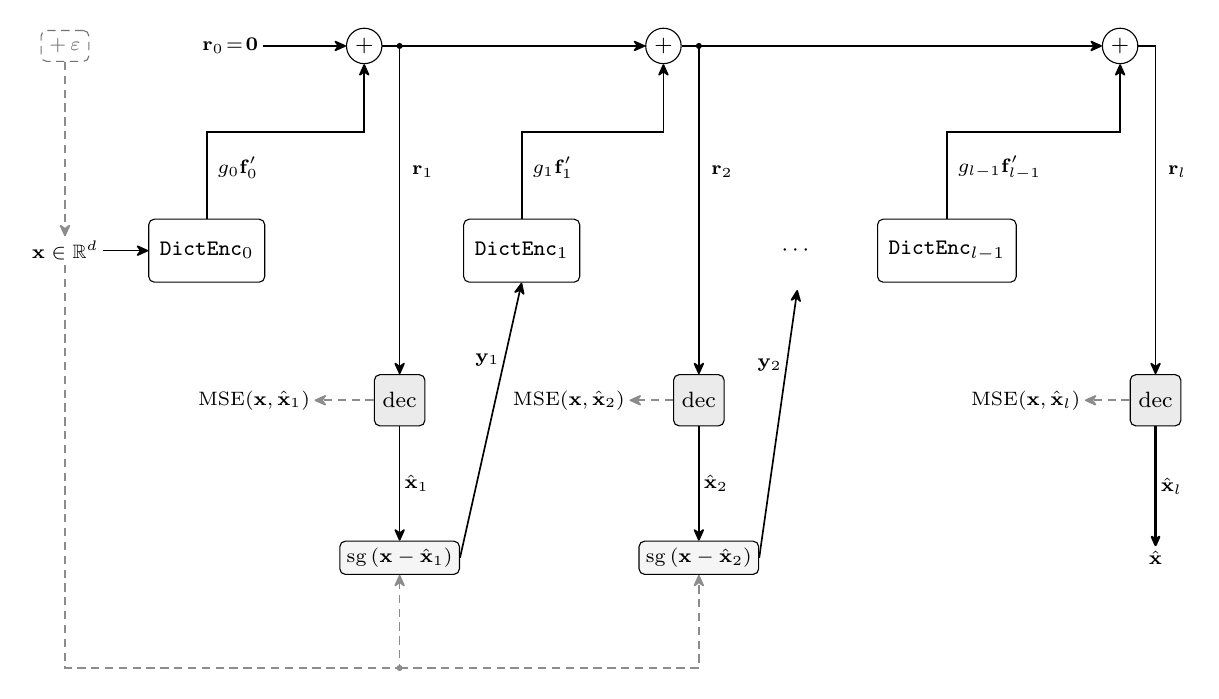
\begin{tikzpicture}[
    font=\footnotesize,
    >={Stealth[round,length=1.8mm,width=1.6mm]},
    blk/.style={draw, rounded corners=2pt, align=center,
                minimum height=8mm, inner xsep=4pt},
    hook/.style={draw, rounded corners=2pt, densely dashed, align=center,
                 inner sep=3pt, font=\scriptsize, black!55},
    dec/.style={draw, rounded corners=2pt, fill=black!8,
                minimum height=6.5mm, inner xsep=3pt},
    cond/.style={draw, rounded corners=2pt, fill=black!4, align=center,
                 inner sep=2.5pt, font=\scriptsize},
    add/.style={draw, circle, minimum size=4.5mm, inner sep=0pt},
    lab/.style={inner sep=1.5pt, font=\scriptsize},
    sig/.style={->, semithick},
    aux/.style={->, densely dashed, semithick, black!45},
  ]

  %% ---- layer row --------------------------------------------------
  \node[lab] (x)  at (-1.5,0) {$\mathbf{x}\in\mathbb{R}^{d}$};
  \node[blk] (D0) at ( 0.3,0) {$\mathtt{DictEnc}_0$};
  \node[blk] (D1) at ( 4.3,0) {$\mathtt{DictEnc}_1$};
  \node      (Dd) at ( 7.8,0) {$\cdots$};
  \node[blk] (DL) at ( 9.7,0) {$\mathtt{DictEnc}_{l-1}$};

  \draw[sig] (x) -- (D0);

  \node[hook] (noise) at (-1.5,2.6) {$+\,\varepsilon$};
  \draw[aux] (noise) -- (x);

  %% ---- residual accumulator (top rail, y = 2.6) --------------------
  \node[add] (A0) at ( 2.3,2.6) {$+$};
  \node[add] (A1) at ( 6.1,2.6) {$+$};
  \node[add] (AL) at (11.9,2.6) {$+$};

  \node[lab] (R0) at (0.6,2.6) {$\mathbf{r}_0\!=\!\mathbf{0}$};
  \draw[sig]      (R0) -- (A0);
  \draw[sig]      (A0) -- (A1);
  \draw[sig]      (A1) -- (AL);
  \draw[semithick] (AL) -- (12.35,2.6);

  %\node[lab] at (8.9,3.05) {$\mathbf{r}\in\mathbb{R}^{e}$: residual accumulator};

  %% ---- per-layer contributions g_l f'_l (enter from below) ----------
  \draw[sig] (D0.north) -- ++(0,1.1) -| (A0.south);
  \draw[sig] (D1.north) -- ++(0,1.1) -| (A1.south);
  \draw[sig] (DL.north) -- ++(0,1.1) -| (AL.south);
  \node[lab,anchor=west] at (0.38,1.05) {$g_0\mathbf{f}'_0$};
  \node[lab,anchor=west] at (4.38,1.05) {$g_1\mathbf{f}'_1$};
  \node[lab,anchor=west] at (9.78,1.05) {$g_{l-1}\mathbf{f}'_{l-1}$};

  %% ---- shared decoder, one decode per prefix -----------------------
  \node[dec] (Y1) at ( 2.75,-1.9) {$\mathrm{dec}$};
  \node[dec] (Y2) at ( 6.55,-1.9) {$\mathrm{dec}$};
  \node[dec] (YL) at (12.35,-1.9) {$\mathrm{dec}$};

  \draw[sig] ( 2.75,2.6) -- (Y1.north);
  \draw[sig] ( 6.55,2.6) -- (Y2.north);
  \draw[sig] (12.35,2.6) -- (YL.north);
  \fill ( 2.75,2.6) circle (1.1pt);
  \fill ( 6.55,2.6) circle (1.1pt);

  \node[lab,anchor=west] at ( 2.85,1.0) {$\mathbf{r}_1$};
  \node[lab,anchor=west] at ( 6.65,1.0) {$\mathbf{r}_2$};
  \node[lab,anchor=west] at (12.45,1.0) {$\mathbf{r}_{l}$};

  %% ---- deep supervision --------------------------------------------
  \node[lab] (L1) at ( 0.9,-1.9) {$\mathrm{MSE}(\mathbf{x},\hat{\mathbf{x}}_1)$};
  \node[lab] (L2) at ( 4.9,-1.9) {$\mathrm{MSE}(\mathbf{x},\hat{\mathbf{x}}_2)$};
  \node[lab] (LL) at (10.7,-1.9) {$\mathrm{MSE}(\mathbf{x},\hat{\mathbf{x}}_{l})$};
  \draw[aux] (Y1.west) -- (L1);
  \draw[aux] (Y2.west) -- (L2);
  \draw[aux] (YL.west) -- (LL);

  %% ---- residual forwarding ------------------------------------------
  \node[cond] (C1) at (2.75,-3.9)
  {$\mathrm{sg}\,(\mathbf{x}-\hat{\mathbf{x}}_1)$};
  \node[cond] (C2) at (6.55,-3.9)
  {$\mathrm{sg}\,(\mathbf{x}-\hat{\mathbf{x}}_2)$};
  \draw[sig] (Y1) -- node[right,lab]{$\hat{\mathbf{x}}_1$} (C1);
  \draw[sig] (Y2) -- node[right,lab]{$\hat{\mathbf{x}}_2$} (C2);

  \draw[sig] (C1.east) -- node[left,lab,pos=0.72]{$\mathbf{y}_1$} (D1.south);
  \draw[sig] (C2.east) -- node[left,lab,pos=0.72]{$\mathbf{y}_2$} (7.8,-0.5);

  %% ---- model output --------------------------------------------------
  \node[lab] (out) at (12.35,-3.9) {$\hat{\mathbf{x}}$};
  \draw[sig,thick] (YL) -- node[right,lab]{$\hat{\mathbf{x}}_{l}$} (out);

  %% ---- x broadcast to every conditioning step -------------------------
  \draw[aux] (x.south) -- (-1.5,-5.3) -- (2.75,-5.3) -- (C1.south);
  \draw[aux] (2.75,-5.3) -- (6.55,-5.3) -- (C2.south);
  \fill[black!45] (2.75,-5.3) circle (1.1pt);

\end{tikzpicture}

}
\caption[\texttt{Ontologizer} architecture]{\textbf{\texttt{Ontologizer} architecture.}
	An \texttt{Ontologizer} consists of $l$ stacked \texttt{DictEnc} layers.
	Each returns a feature vector $\mathbf{f}'_\ell\in\mathbb{R}^{e}$,
	which is written, scaled by its input's gain $g_\ell$, to a residual
	accumulator $\mathbf{r}$.
	For each layer $\ell = 0, \dots, l-1$,
	$\mathbf{r}_\ell = \mathbf{r}_{\ell-1} + g_\ell\,\mathbf{f}'_\ell$ with
	$\mathbf{r}_{-1} := \mathbf{0}$; a stop-gradient variant
	($\mathrm{sg}$ on $\mathbf{r}_{\ell-1}$, available but off in the live
	configuration) would prevent gradient communication between layers.
	$\mathrm{dec}$ is a linear decoder with shape $\mathbb{R}^{d \times e}$.
	It uses deep supervision to obtain a coarse-to-fine representation where
	the component encoded by previous layers is inaccessible to later layers.
	At each layer $\ell$, $\hat{\mathbf{x}}_\ell = \mathrm{dec}(\mathbf{r}_\ell)$.
	The same decoder is shared by all layers.
	The component left unexplained after layer $\ell$ is given by
	$\mathbf{y}_\ell = \mathbf{x} - \hat{\mathbf{x}}_\ell$.
	The input to layer $\ell+1$ is given by
	$\tilde{\mathbf{y}}_\ell
	  = \mathbf{y}_\ell / \mathrm{L2}(\mathbf{y}_\ell) \oplus [1]$
	where $\mathrm{L2}$ is the unit norm. This prevents exploding gradients from repeated
	application of bilinear layers, as each scales its input by $\lVert\cdot\rVert^{2}$.
	A constant coordinate $[1]$ is appended, giving a dimension of $d+1$.
	This prevents the sign information of $\mathbf{y}_\ell$ from being lost
	by the bilinear transformation.
	Effectively, it adds a bias to an otherwise unbiased linear form
	while preserving eigendecomposition.

	$\mathrm{MSE}(\mathbf{x},\mathrm{dec}(\mathbf{r}_\ell))$ is computed separately for each layer.

	The input-noise hook drawn on $\mathbf{x}$ is available but disabled
	in every model reported here.
}
\label{fig:onto-stack}
\end{figure}

\subsubsection{DictEnc}
\label{sec:dictenc}
Each $\dictenc$ consists of a multihead bilinear classifier
($\bilinearblock$) with weights
$[\mathsf{W}, \mathsf{V}] \in \mathbb{R}^{2 \times h \times k \times d}$
($d+1$ after the first layer, see Eq.~\ref{eq:y_norm})
and a multihead linear dictionary ($\dictblock$)
with weights $\mathsf{D} \in \mathbb{R}^{h \times k \times e}$.
It accepts a vector $\mathbf{x} \in \mathbb{R}^{d}$,
which may be a residual from a previous layer.
Algorithm~\ref{alg:dictenc} gives one layer's training pass, and
Algorithm~\ref{alg:ontologizer} the stack and its loss.

\begin{algorithm}[tp]
	\caption{$\dictenc$, one layer, in training (\texttt{DictEnc.withStats}).
	Without the router, $S$ is all ones and $\mathrm{L1}_S = 0$; without
	fibers there are no coordinates $\mathsf{C}$; without
	\texttt{resid\_gain} the input is not split and $g = 1$.}
	\label{alg:dictenc}
	\DontPrintSemicolon

	\KwIn{accumulator $R \in \mathbb{R}^{b \times e}$; layer input
		$E \in \mathbb{R}^{b \times d'}$, whose last $c$ coordinates are
		constant (\texttt{resid\_const})}
	\KwData{bilinear classifier (Eq.~\ref{eq:bilinearblock}); router
		(\texttt{scaled}); fiber readouts $A_i \in \mathbb{R}^{r \times d'}$;
		$\dictblock$ (Algorithm~\ref{alg:dictblock})}
	\Hyper{logit noise $\sigma_K$; fiber bound $\beta$; the
		$\dictblock$ hyperparameters}
	\KwOut{accumulator $R$; assignments
		$\mathsf{P} \in \mathbb{R}^{b \times h \times k}$; statistics
		row $\mathbf{m}$ (Eq.~\ref{eq:stats})}

	\Begin{
		$g_n \leftarrow \mathrm{sg}\big[\lVert E_{n,1:d'-c}\rVert\big]$;\quad
			$\mathbf{u}_n \leftarrow \big[E_{n,1:d'-c}/g_n;\,
			E_{n,d'-c+1:d'}\big]$
			\tcp*{gain and shape}
		$\mathsf{K}, \mathrm{L1}_K \leftarrow
			\mathrm{classifier}(\mathbf{u})$
			\tcp*{L1 of the gate factor}
		$\mathsf{K} \leftarrow \mathrm{noise}_K(\mathsf{K})$
			\tcp*{Eq.~\ref{eq:noise_normal} or~\ref{eq:noise_batchnorm}}
		\eIf{router}{
			$S, \mathrm{L1}_S \leftarrow \mathrm{router}(\mathbf{u})$;\quad
				$S \leftarrow \lvert S \rvert$
				\tcp*{unless \texttt{router\_signed}}
		}{
			$S \leftarrow \mathbf{1}$;\quad $\mathrm{L1}_S \leftarrow 0$\;
		}
		$\mathbf{c}_{ni} \leftarrow \beta \tanh(A_i \mathbf{u}_n / \beta)$
			\tcp*{fiber coordinates, Eq.~\ref{eq:fiber}}
		$F', \mathsf{P}, (\mathrm{L1}, H, \mathrm{cossim}_b,
			\mathbb{E}\kappa, \max\kappa, \mathrm{KL}_m, \sigma)
			\leftarrow \dictblock(\mathsf{K}, S, \mathsf{C})$\;
		$\mathrm{KL}_{\mathrm{pwak}}, \mathrm{L2}_{\mathrm{pwak}}
			\leftarrow \mathrm{pwak}(\mathsf{P}, \mathbf{u})$
			\tcp*{zero unless enabled}
		$R_n \leftarrow R_n + g_n\,\mathbf{f}'_n$
			\tcp*{the contribution, at the input's gain}
		\Return{$R$, $\mathsf{P}$,
			$\mathbf{m} = (\mathrm{L1}_K, \mathrm{L1}, H, \mathrm{cossim}_b,
			\mathbb{E}\kappa, \max\kappa, \mathrm{KL}_m,
			\mathrm{KL}_{\mathrm{pwak}}, \mathrm{L2}_{\mathrm{pwak}},
			\mathrm{L1}_S, \sigma)$}\;
	}
\end{algorithm}


\begin{figure}[tp]
\centering
\resizebox{\linewidth}{!}{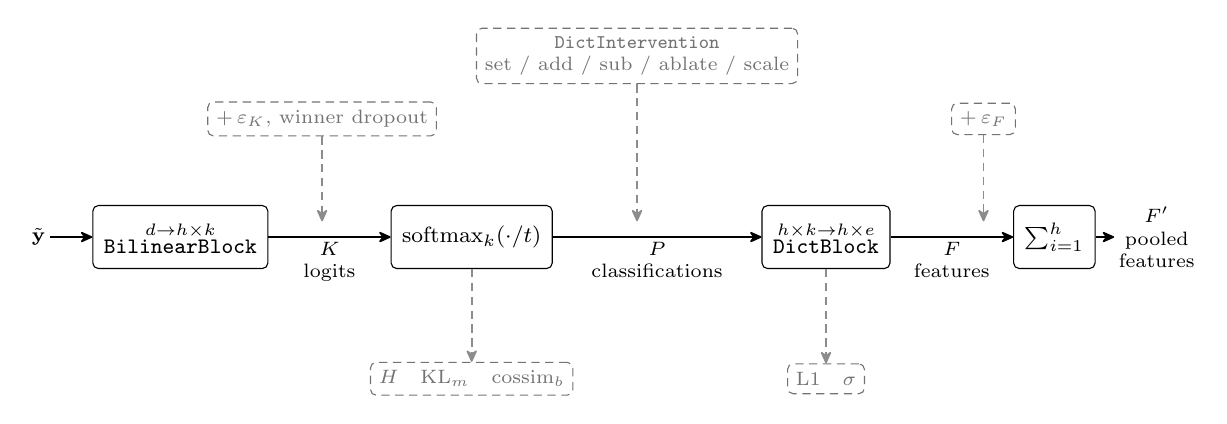
\begin{tikzpicture}[
    font=\footnotesize,
    >={Stealth[round,length=1.8mm,width=1.6mm]},
    blk/.style={draw, rounded corners=2pt, align=center,
                minimum height=8mm, inner xsep=4pt},
    hook/.style={draw, rounded corners=2pt, densely dashed, align=center,
                 inner sep=3pt, font=\scriptsize, black!55},
    lab/.style={inner sep=1.5pt, font=\scriptsize, align=center},
    sig/.style={->, semithick, align=center},
    aux/.style={->, densely dashed, semithick, black!45},
  ]

  %% ---- main chain ----------------------------------------------------
  \node[lab] (E)  at (-0.6,0) {$\tilde{\mathbf{y}}$};
  \node[blk] (CL) at ( 1.2,0) {$\bilinearblock^{d \to h \times k}$};
  \node[blk] (SM) at ( 4.9,0) {$\mathrm{softmax}_k(\cdot/t)$};
  \node[blk] (DB) at ( 9.4,0) {$\dictblock^{h \times k \to h \times e}$};
  \node[blk] (SU) at (12.3,0) {$\sum^{h}_{i=1}$};
  \node[lab] (F)  at (13.6,0) {$F'$\\ pooled\\ features};

  \draw[sig] (E)  -- (CL);
  \draw[sig] (CL) -- node[below,lab]{$K$\\ logits}   (SM);
  \draw[sig] (SM) -- node[below,lab]{$P$\\ classifications}   (DB);
  \draw[sig] (DB) -- node[below,lab]{$F$\\ features} (SU);
  \draw[sig] (SU) -- (F);

  %% ---- training-time hooks and the intervention interface (above) ----
  \node[hook] (nk) at (3.0,1.5) {$+\,\varepsilon_K$,\ winner dropout};
  \node[hook] (iv) at (7.0,2.3) {\texttt{DictIntervention}\\
                                 set / add / sub / ablate / scale};
  \node[hook] (nf) at (11.4,1.5) {$+\,\varepsilon_F$};
  \draw[aux] (nk) -- (3.0,0.20);
  \draw[aux] (iv) -- (7.0,0.20);
  \draw[aux] (nf) -- (11.4,0.20);

  %% ---- where each regulariser attaches (below) -----------------------
  \node[hook] (lp) at (4.9,-1.8)
    {$H$\quad $\mathrm{KL}_m$\quad $\mathrm{cossim}_b$};
  \node[hook] (lf) at (9.4,-1.8)
    {$\mathrm{L1}$\quad $\sigma$};
  \draw[aux] (SM.south) -- (lp);
  \draw[aux] (DB.south) -- (lf);

\end{tikzpicture}

}
\caption[\texttt{DictEnc} architecture]{\textbf{\texttt{DictEnc} architecture.}
	Dashed lines above indicate perturbations to the data,
	including noising and causal interventions.
	Dashed lines below indicate statistics used as tuneable auxiliary loss functions.
	Each \texttt{DictEnc} consists of a multihead bilinear classifier
	(see §\ref{sec:bilinear})
	and a multihead linear dictionary (see §\ref{sec:dict}).
	It accepts a vector $\mathbf{x} \in \mathbb{R}^{d}$,
	which may be a residual from a previous layer.
	Optional noise terms $\varepsilon_K$ and $\varepsilon_F$ may be added
	(see §\ref{sec:noise}).
	Winner dropout sets each head's largest logit to $-\infty$
	with probability $p_{\mathrm{drop}}$.

	Soft assignments $P$ are given by $\mathrm{softmax}_{k}(K/t)$
	(see §\ref{sec:labels}).
	The architecture provides methods for causal interventions on assignments.
	From $P$ we collect per-sample entropy $H$ (Eq.~\ref{eq:entropy}),
	between-sample similarity $\mathrm{cossim}_b$ (Eq.~\ref{eq:cossim_b}),
	and batch mean entropy $\mathrm{KL}_m$ (Eq.~\ref{eq:KL}).

	A $\dictblock$ accepts assignments
	$P \in \mathbb{R}^{h \times k}$
	and returns features $F \in \mathbb{R}^{h \times e}$ (Eq.~\ref{eq:dictblock}).
	From $P$ and the atoms we collect the heads' support overlap $\omega$
	(Eq.~\ref{eq:support}), and from $F$ the sparsity penalty $\mathrm{L1}$
	(Eq.~\ref{eq:L1}).
	$F$ is summed over the head dimension to obtain
	pooled features $\mathbf{f}' \in \mathbb{R}^{e}$, which are added to
	the accumulator $\mathbf{r}$.
}
\label{fig:dictenc}
\end{figure}

\subsubsection{Classifier}
\label{sec:bilinear}
A $\bilinearblock$ accepts inputs $\mathbf{x} \in \mathbb{R}^d$.
It returns logits $K \in \mathbb{R}^{h \times k}$ given by

\begin{equation}
	\bilinearblock([\mathsf{W},\mathsf{V}],\mathbf{x}) :=
	\left(\sum^{d}_{q=1}W_{\cdot,\cdot,q}\,x_q\right)
	 \odot \left(\sum^{d}_{q=1}V_{\cdot,\cdot,q}\,x_q\right)
	 \label{eq:bilinearblock}
\end{equation}

An optional noise term $\varepsilon_K$ may be added.
Winner dropout sets each head's largest logit to $-\infty$
with probability $p_{\mathrm{drop}}$.

\subsubsection{Assignments}
\label{sec:labels}
Soft assignments $P$ are given by $\mathrm{softmax}_{k}(K/t)$
where $t$ is a temperature hyperparameter. Annealing it sharpens the
assignments; each model's schedule is in Appendix~\ref{app:configs}.
The architecture provides methods for causal interventions on assignments.
From $P$ we collect per-sample entropy $H$, in bits, so a head
saturates at $\log_2 k = 5$ bits,

\begin{equation}
	\mathrm{entropy}_k(\mathbf{p}) :=
	-\sum^{k}_{j=1}p_{j}\log_2 p_{j},
	\qquad
	H := \mathbb{E}_{n}\,\mathbb{E}_{i}\!\left[
	\mathrm{entropy}_k(\mathbf{p}_{ni})\right]
	\label{eq:entropy}
\end{equation}

between-sample similarity $\mathrm{cossim}_b$, the mean absolute cosine
similarity of the per-head features $\mathsf{F}$ over all ordered pairs
of samples,

\begin{equation}
	\mathrm{cossim}_b(\mathsf{P}) :=
	\mathbb{E}_{n,n'}\left[\left\lvert
	\frac{\langle \mathbf{f}_{n}, \mathbf{f}_{n'}\rangle}
	     {\lVert \mathbf{f}_{n}\rVert \lVert \mathbf{f}_{n'}\rVert}
	\right\rvert\right],
	\qquad
	\langle \mathbf{f}_{n}, \mathbf{f}_{n'}\rangle
	= \sum^{h}_{i=1}\mathbf{p}_{ni}^{\top}G_{i}\,\mathbf{p}_{n'i}
	\label{eq:cossim_b}
\end{equation}

where $\mathbf{f}_{ni} := \mathsf{F}_{ni\cdot} \in \mathbb{R}^{e}$ is
head $i$'s feature vector for sample $n$,
$\mathbf{f}_n = \map_{i=1}^{h}\mathbf{f}_{ni}$ is their concatenation,
and
$G_i = \lvert D_{i}\rvert \lvert D_{i}\rvert^{\top} \in \mathbb{R}^{k \times k}$
is head $i$'s dictionary Gram, with $D_i := \mathsf{D}_{i\cdot\cdot}$ its
$k \times e$ dictionary. The implementation evaluates
Equation~\ref{eq:cossim_b} in entry space through the $G_i$ rather than
materializing $\mathsf{F}$; the two are identical in value and gradient,
but $\mathcal{O}(hk^2e + b^2hk)$ instead of $\mathcal{O}(b^2he)$.

Finally, $\mathrm{KL}_m$ is the divergence of the batch-mean assignment
vector from uniform, in bits, averaged over heads.

\begin{equation}
	\mathrm{KL}_m(\mathsf{P}) := \mathbb{E}_{i}\!\left[\log_2 k -
	\mathrm{entropy}_k\!\left(\bar{\mathbf{p}}_i\right)\right],
	\qquad
	\bar{\mathbf{p}}_i := \mathbb{E}_{n}\,[\mathbf{p}_{ni}]
	\label{eq:KL}
\end{equation}

In practice $H$ is not needed, as including a
$\mathrm{cossim}_b$ loss also minimizes $H$.
$\mathrm{KL}_m$ serves to anchor the batch mean of each assignment vector
$\mathbf{p}_{ni}$ to a uniform distribution.
This results in a uniform $\mathbf{p}_{ni}$ code corresponding
to a maximally generic feature vector.

\subsubsection{Dictionary}
\label{sec:dict}
A $\dictblock$ accepts assignments
$P \in \mathbb{R}^{h \times k}$
and returns features $F \in \mathbb{R}^{h \times e}$, whose row
$\mathbf{f}_i$ is head $i$'s output, given by

\begin{equation}
	\dictblock(\mathsf{D},P)_{i\cdot} = \mathbf{f}_i :=
	\sum^{k}_{j=1} p_{ij}\,\mathbf{a}_{ij},
	\qquad
	\mathbf{a}_{ij} := \lvert \mathsf{D}_{ij\cdot}\rvert
	\label{eq:dictblock}
\end{equation}

where the atom $\mathbf{a}_{ij}$ is the absolute value of head $i$'s
dictionary row for entry $j$ ($\mathsf{D}_{ij\cdot}$ itself when the
dictionary is signed). Because atoms are absolute values
and $p_{ij} \in [0,1]$, features are strictly additive.
Algorithm~\ref{alg:dictblock} gives the full training pass, with the
regularizing perturbations and statistics around this lookup.

\begin{algorithm}[tp]
	\caption{$\dictblock$ in training (\texttt{DictBlock.withStats}). At
	inference the four stochastic steps (revival, winner dropout, head
	dropout, fiber dropout) and the feature noise are skipped. Every
	statistic is stop-gradiented unless its loss term is enabled.}
	\label{alg:dictblock}
	\DontPrintSemicolon

	\KwIn{logits $\mathsf{K} \in \mathbb{R}^{b \times h \times k}$;
		router scales $S \in \mathbb{R}_{\ge 0}^{b \times h}$ (all ones
		without a router); fiber coordinates
		$\mathsf{C} \in \mathbb{R}^{b \times h \times r}$ (none without
		fibers)}
	\KwData{dictionary $\mathsf{D} \in \mathbb{R}^{h \times k \times e}$;
		fiber bases $U_{ij} \in \mathbb{R}^{e \times r}$}
	\Hyper{temperature $t$; feature noise $\sigma_F$; winner dropout
		$p_{\mathrm{drop}}$; revival rate $p_{\mathrm{rev}}$ and threshold
		$\rho$; head dropout $p_{\mathrm{head}}$; fiber dropout
		$p_{\mathrm{fib}}$; entries kept per head $k_{\mathrm{sel}}$
		($1$ under \texttt{ste}/\texttt{argmax}, $m$ under
		\texttt{top}$m$, $k$ under softmax)}
	\KwOut{pooled features $F' \in \mathbb{R}^{b \times e}$; assignments
		$\mathsf{P} \in \mathbb{R}^{b \times h \times k}$; statistics
		$(\mathrm{L1}, H, \mathrm{cossim}_b, \mathbb{E}_i\kappa_i,
		\max_i \kappa_i, \mathrm{KL}_m, \sigma)$}

	\Begin{
		$\mathbf{d}_{ij} \leftarrow \lvert \mathsf{D}_{ij\cdot} \rvert$
			\tcp*{atoms; $\mathsf{D}_{ij\cdot}$ itself if signed}
		\If(\tcp*[f]{revive starved entries}){$k_{\mathrm{sel}} < k$}{
			$u_{ij} \leftarrow \mathbb{E}_n\,\mathbf{1}\{K_{nij}$ is among
				head $i$'s top $k_{\mathrm{sel}}$ logits$\}$\;
			\ForEach{$(n,i)$ with probability $p_{\mathrm{rev}}$}{
				draw $j$ uniformly from $\{j : u_{ij} <
					\rho\,k_{\mathrm{sel}}/k\}$, if any\;
				$K_{nij} \leftarrow \max_{j'} K_{nij'}$
					\tcp*{tie the leader}
			}
		}
		\ForEach(\tcp*[f]{winner dropout}){$(n,i)$ with probability
			$p_{\mathrm{drop}}$}{
			$K_{n,i,\arg\max_j K_{nij}} \leftarrow -\infty$\;
		}
		$\mathsf{P} \leftarrow \mathrm{select}_k(\mathsf{K}/t)$
			\tcp*{softmax, top-$m$ or straight-through}
		$H \leftarrow \mathbb{E}_{n,i}\,\mathrm{entropy}_k(\mathbf{p}_{ni})$
			\tcp*{Eq.~\ref{eq:entropy}}
		$\bar{\mathbf{p}}_i \leftarrow \mathrm{sg}[\mathbb{E}_n\,
			\mathbf{p}_{ni}]$ \tcp*{head origin}
		\ForEach(\tcp*[f]{head dropout}){$(n,i)$}{
			$\mathbf{p}'_{ni} \leftarrow \bar{\mathbf{p}}_i$ with
				probability $p_{\mathrm{head}}$, else
				$\bar{\mathbf{p}}_i + (\mathbf{p}_{ni} - \bar{\mathbf{p}}_i)
				/ (1 - p_{\mathrm{head}})$\;
		}
		\ForEach(\tcp*[f]{fiber dropout}){$(n,i)$ with probability
			$p_{\mathrm{fib}}$}{
			$\mathbf{c}_{ni} \leftarrow \mathbf{0}$\;
		}
		$\mathbf{f}_{ni} \leftarrow S_{ni} \sum_{j} p'_{nij}\,
			\mathbf{d}_{ij}$ \tcp*{Eq.~\ref{eq:dictblock}; interventions act
			on $\mathbf{p}'$}
		$\tilde{\mathsf{F}} \leftarrow \mathrm{noise}_{\mathrm{featvar}}
			(\mathsf{F})$ \tcp*{Eq.~\ref{eq:noise_featvar}}
		$\mathrm{cossim}_b \leftarrow \mathrm{cossim}_b(\mathsf{P})$
			\tcp*{Eq.~\ref{eq:cossim_b}, through the Grams}
		$\kappa_i \leftarrow \mathbb{E}_{j \ne j'}
			\cos(\mathbf{d}_{ij}, \mathbf{d}_{ij'})$
			\tcp*{within-head row cosine}
		$\mathrm{KL}_m \leftarrow \mathbb{E}_i \left[\log_2 k -
			\mathrm{entropy}_k(\bar{\mathbf{p}}_i)\right]$
			\tcp*{Eq.~\ref{eq:KL}}
		$\mathbf{s}_i \leftarrow \sum_j \bar{p}_{ij}\,
			\lvert\mathbf{d}_{ij}\rvert$;\quad
			$\sigma \leftarrow \mathbb{E}_{i \ne i'}
			\cos(\mathbf{s}_i, \mathbf{s}_{i'})$
			\tcp*{support overlap}
		$\mathrm{L1} \leftarrow \mathbb{E}_n \sum_i
			\lVert \tilde{\mathbf{f}}_{ni} \rVert_1$\;
		$\mathbf{f}'_n \leftarrow \sum_i \tilde{\mathbf{f}}_{ni}$
			\tcp*{concatenated, not summed, under $\mathtt{ConcatDictBlock}$}
		\If(\tcp*[f]{Eq.~\ref{eq:fiber}, then any norm cap}){fibers}{
			$\mathbf{f}'_n \leftarrow \mathbf{f}'_n + \sum_i S_{ni}
				\sum_j p'_{nij}\,U_{ij}\,\mathbf{c}_{ni}$\;
		}
		\Return{$F'$, $\mathsf{P}$,
			$(\mathrm{L1}, H, \mathrm{cossim}_b, \mathbb{E}_i\kappa_i,
			\max_i \kappa_i, \mathrm{KL}_m, \sigma)$}\;
	}
\end{algorithm}


From the assignments and the atoms we collect the heads' support overlap
$\omega$, the mean cosine over ordered pairs of distinct heads between
their usage-weighted coordinate profiles $\boldsymbol{\pi}_i$,

\begin{equation}
	\boldsymbol{\pi}_i := \sum^{k}_{j=1} \bar{p}_{ij}\,
	\lvert \mathbf{a}_{ij}\rvert,
	\qquad
	\omega := \mathbb{E}_{i \neq i'}\,
	\frac{\langle \boldsymbol{\pi}_i, \boldsymbol{\pi}_{i'}\rangle}
	     {\lVert \boldsymbol{\pi}_i\rVert \lVert \boldsymbol{\pi}_{i'}\rVert}
	\label{eq:support}
\end{equation}

with $\bar{\mathbf{p}}_i$ the batch-mean assignment of
Equation~\ref{eq:KL}. The overlap is zero exactly when no two heads share
a coordinate of the dictionary space and one when every head uses the
same coordinates in the same proportions (Section~\ref{sec:disjoint}). It
costs
$\mathcal{O}(hke + h^2e)$, independent of the batch. Weighting by usage
keeps dead entries out of it and gives the classifier a gradient path.
We also collect the sparsity penalty $\mathrm{L1}$ after the noise
$\varepsilon_F$ is added, $\tilde{\mathsf{F}} := \mathsf{F} +
\varepsilon_F$. $\mathrm{L1}$ is the batch mean of each sample's norm, so
it does not change with $b$ but scales with $h$ and $e$; its loss weight
is correspondingly small.

\begin{equation}
	\mathrm{L1}(\tilde{\mathsf{F}}) :=
	\frac{1}{b}\sum^{b}_{n=1}\sum^{h}_{i=1}\sum^{e}_{q=1}
	\lvert \tilde{f}_{niq}\rvert
	\label{eq:L1}
\end{equation}

$\mathrm{L1}$ tends to decrease with only $\mathrm{MSE}$ loss, but
incorporating it into the loss speeds up convergence.

\paragraph{Disjoint support}
\label{sec:disjoint}
Between heads, orthogonality of nonnegative features is not a rotation
constraint but a support-partition constraint. Every $\mathbf{f}_{ni}$
lies in the nonnegative orthant of
$\mathbb{R}^e$: the dictionary contributes $\lvert \mathsf{D} \rvert \geq 0$ and
the assignments $P \geq 0$. For nonnegative $\mathbf{v}, \mathbf{v}'$ the
inner product $\langle \mathbf{v},\mathbf{v}'\rangle = \sum_q v_q v'_q$ is
a sum of nonnegative terms, so it vanishes if and only if every term
does,

\begin{equation}
	\langle \mathbf{v},\mathbf{v}'\rangle = 0
	\iff
	\mathrm{supp}(\mathbf{v}) \cap \mathrm{supp}(\mathbf{v}') = \emptyset
	\label{eq:disjoint}
\end{equation}

Signed vectors admit no such conclusion: there orthogonality is
cancellation, and two vectors with identical support can be orthogonal.
The support overlap of Equation~\ref{eq:support} sidesteps this. It
compares the absolute values of the atoms, which have disjoint supports
exactly when they are orthogonal whatever the atoms' signs, so it
measures disjointness under a signed dictionary too; and it is computed
from the atoms and the batch-mean assignment rather than from noised
features, which leave the orthant and the argument with it.

The constraint binds the dictionary, not merely one sample's features.
Because the assignments are a softmax, $p_{nij} > 0$ for every entry, and expanding
Equation~\ref{eq:dictblock} gives

\begin{equation}
	\langle \mathbf{f}_{ni},\mathbf{f}_{ni'}\rangle =
	\sum^{k}_{j=1}\sum^{k}_{j'=1} p_{nij}\,p_{ni'j'}
	\left\langle \mathbf{a}_{ij}, \mathbf{a}_{i'j'} \right\rangle
	\label{eq:cross_head}
\end{equation}

a strictly positive combination of all $k^2$ cross-head atom overlaps.
A single sample on which heads $i$ and $i'$ are orthogonal therefore
forces $\langle \mathbf{a}_{ij}, \mathbf{a}_{i'j'}\rangle = 0$ for every
pair of atoms $(j,j')$: the two heads own disjoint blocks of coordinates
as a property of $\mathsf{D}$, holding for all inputs rather than on the
data that happened to be measured. That is the premise a static reading
of the dictionary needs, and it is stronger than what any signed-feature
architecture can ask for. The budget is not tight either. In the softmax
configuration (Table~\ref{tab:cfg-softmax}), $h{=}32$ heads partitioning
$e{=}2048$ coordinates leaves
64 dimensions per head to hold $k{=}32$ atoms, which need not be
disjoint from each other within a head; head-disjointness is most of
what the width $e > d$ buys.

Two different orthogonalities are in play and only the between-head one
is architectural. Disjoint support assigns each head a block of
coordinates; \emph{within} a head the $k$ atoms are contrastive
alternatives spread apart inside that block
(Figure~\ref{fig:head-simplex}). Section~\ref{sec:prelim-orth} measures
the second. Neither is guaranteed at convergence: $\omega$ is a penalty,
and the geometry is built to make a support partition the cheap solution
rather than to force one. Measured on the trained models, the cheap
solution was not taken: the within-head orthogonality holds, and no model
partitions its coordinates between heads (Appendix~\ref{sec:support}).
Under $\mathtt{ConcatDictBlock}$ heads write disjoint slices by
construction and $\omega$ is identically zero.

We add noise $\varepsilon_F$ to $F$, then sum over the head dimension to obtain
pooled features $\mathbf{f}' \in \mathbb{R}^{e}$, which are added to the
accumulator $\mathbf{r}$.

\begin{equation}
	\mathbf{f}' = \sum^{h}_{i=1}\tilde{\mathbf{f}}_{i}
	\label{eq:pool}
\end{equation}

\begin{figure}[tp]
\centering
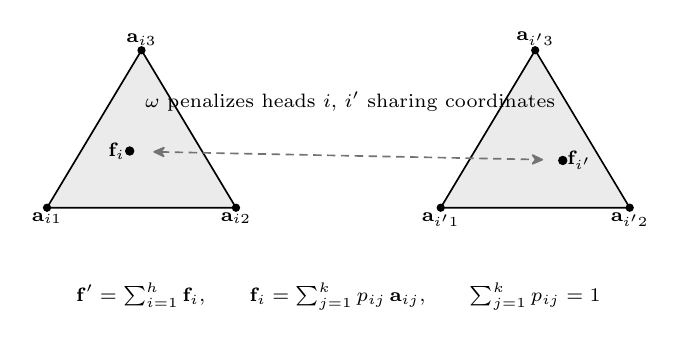
\begin{tikzpicture}[
    font=\footnotesize,
    >={Stealth[round,length=1.8mm,width=1.6mm]},
    lab/.style={inner sep=1.5pt, font=\scriptsize},
  ]
  %% ---- head i --------------------------------------------------------
  \fill[black!8]   (0,0) -- (2.4,0) -- (1.2,2.0) -- cycle;
  \draw[semithick] (0,0) -- (2.4,0) -- (1.2,2.0) -- cycle;
  \fill (0,0)     circle (1.5pt) node[below,lab]{$\mathbf{a}_{i1}$};
  \fill (2.4,0)   circle (1.5pt) node[below,lab]{$\mathbf{a}_{i2}$};
  \fill (1.2,2.0) circle (1.5pt) node[above,lab]{$\mathbf{a}_{i3}$};
  \fill (1.05,0.72) circle (1.7pt) node[left,lab]{$\mathbf{f}_i$};

  %% ---- head i' ------------------------------------------------------
  \fill[black!8]   (5.0,0) -- (7.4,0) -- (6.2,2.0) -- cycle;
  \draw[semithick] (5.0,0) -- (7.4,0) -- (6.2,2.0) -- cycle;
  \fill (5.0,0)   circle (1.5pt) node[below,lab]{$\mathbf{a}_{i'1}$};
  \fill (7.4,0)   circle (1.5pt) node[below,lab]{$\mathbf{a}_{i'2}$};
  \fill (6.2,2.0) circle (1.5pt) node[above,lab]{$\mathbf{a}_{i'3}$};
  \fill (6.55,0.60) circle (1.7pt) node[right,lab]{$\mathbf{f}_{i'}$};

  \draw[<->, densely dashed, semithick, black!55] (1.35,0.71) -- (6.30,0.61);
  \node[lab] at (3.85,1.35)
    {$\omega$ penalizes heads $i$, $i'$ sharing coordinates};

  \node[lab, anchor=north, align=center] at (3.7,-0.9)
  {$\mathbf{f}'=\sum^h_{i=1} \mathbf{f}_i$,\qquad
  $\mathbf{f}_i=\sum^k_{j=1} p_{ij}\,\mathbf{a}_{ij}$,\qquad $\sum^k_{j=1} p_{ij}=1$};
\end{tikzpicture}


\caption[Per-head geometry]{\texttt{DictBlock} \textbf{head geometry} for $h{=}2$, $k{=}3$.
	The output space of a head $i$ forms a simplex with its atoms
	$\mathbf{a}_{ij}$, the rows of $\lvert D_i\rvert$, as the vertices.
	The atoms form the spanning set of the
	feature space. Any $\mathbf{f}_i$ must be a linear combination of them.
	As $F$ becomes sparser, these vectors become more approximately
	orthogonal, allowing them to be treated as a basis.
	The assignment code $P$ corresponds to soft assignments to mutually
	contrastive categories rather than independently firing features.
	Because elements of $P$, $p_{ij} \in [0,1]$,
	outputs must be within the convex hull of head $i$'s atoms.
	Because $\lvert \mathsf{D}\rvert\geq0$ and $P\geq0$, $F\geq0$;
	therefore $\cos(\mathbf{f}_i, \mathbf{f}_{i'}) \in [0,1]$, and driving the support
	overlap $\omega$ to zero asks the heads to partition the
	coordinates of $\mathbb{R}^e$ between them
	(Section~\ref{sec:disjoint}).
}
\label{fig:head-simplex}
\end{figure}

\subsubsection{Decoder}
\label{sec:decoder}
Each $\dictenc$ output $\mathbf{f}'_\ell$, scaled by its input's gain
$g_\ell$, is added to an accumulator $\mathbf{r}$.

\begin{equation}
	\mathbf{r}_\ell = \sum_{\ell'=0}^{\ell} g_{\ell'}\,\mathbf{f}'_{\ell'},
	\qquad
	g_\ell := \mathrm{sg}\!\left[\mathrm{L2}(\mathbf{y}_{\ell-1})\right]
\end{equation}

Under \texttt{resid\_gain} a layer classifies only the direction of its
input, so the gain carries the magnitude it cannot see; without it
$g_\ell = 1$. Layer 0's input is the encoded input itself,
$\mathbf{y}_{-1} := \mathbf{x}$, whose gain is identically 1 on unit-norm
SONAR embeddings.

A single-layer unbiased linear decoder $\mathrm{dec}$ projects
$\mathbf{r}_\ell$ back to the input space $\mathbb{R}^d$. Weights
$W_{\mathrm{dec}} \in \mathbb{R}^{d \times e}$
are shared for all $\mathtt{DictEnc}_\ell$.

\begin{equation}
	\hat{\mathbf{x}}_\ell = W_{\mathrm{dec}}\,\mathbf{r}_\ell
	\label{eq:dec}
\end{equation}

The residual $\mathbf{y}_\ell$ is given by $\mathbf{x} - \hat{\mathbf{x}}_\ell$, stop-gradiented so that
lower layers cannot write a communication code into the residual instead
of reducing it.
It is normalized by the unit norm $\mathrm{L2}$, with $\epsilon$ the
floating-point epsilon of the working dtype.

\begin{equation}
	\mathbf{y}_\ell = \mathrm{sg}\!\left[\mathbf{x} - \hat{\mathbf{x}}_\ell\right],
	\qquad
	\mathrm{L2}(\mathbf{y}) := \sqrt{\sum^{d}_{q=1} y_q^2}
	\label{eq:L2}
\end{equation}

\begin{equation}
	\tilde{\mathbf{y}}_\ell =
	\frac{\mathbf{y}_\ell}{\mathrm{L2}(\mathbf{y}_\ell) + \epsilon} \oplus [1]
	\label{eq:y_norm}
\end{equation}

A constant coordinate $[1]$ is appended, giving a dimension of $d+1$.
This prevents the sign information of $\mathbf{y}_\ell$ from being lost
by the bilinear transformation.
Effectively, it adds a bias to an otherwise unbiased linear form
while preserving eigendecomposition.

\subsubsection{Noise}
\label{sec:noise}
Noise is added to $X$, $\mathsf{K}$, and $\mathsf{F}$, controlled by
hyperparameters $\sigma_X$, $\sigma_K$, and $\sigma_F$. Each draws a
standard normal of the same shape as its target,

\begin{equation}
	\varepsilon \sim \mathcal{N}(0,1)
\end{equation}

and scales it three different ways. Classifier logits take unscaled
Gaussian noise,

\begin{equation}
	\mathrm{noise}_{\mathrm{normal}}(\mathsf{K}) :=
	\mathsf{K} + \sigma_K\varepsilon
	\label{eq:noise_normal}
\end{equation}

inputs take noise proportional to their own norm, so the scale is a
fraction of signal magnitude rather than an absolute quantity,

\begin{equation}
	\mathrm{noise}_{\mathrm{batchnorm}}(X) := X + \sigma_X\,\varepsilon
	\odot \frac{\mathrm{sg}\!\left[\mathrm{L2}(X)\right]}{\sqrt{d}}
	\label{eq:noise_batchnorm}
\end{equation}

and features take noise proportional to each feature's standard
deviation across the batch.

\begin{equation}
	\mathrm{noise}_{\mathrm{featvar}}(\mathsf{F}) := \mathsf{F} +
	\sigma_F\,\varepsilon \odot \mathrm{sg}\!\left[
	\sqrt{\mathrm{var}_n(\mathsf{F}) + \epsilon}\right]
	\label{eq:noise_featvar}
\end{equation}

Here $\mathrm{L2}(X)$ is the per-sample norm of
Equation~\ref{eq:L2}, broadcast over $d$. Both scales are
stop-gradiented: without $\mathrm{sg}$ the model could evade its own
noise by shrinking feature variance, and the $\epsilon$ inside the root
guards the $0/0$ gradient where a feature's batch variance underflows to
exactly zero. Because $\sigma_K$ enters the softmax as $\sigma_K/t$,
holding it constant under a falling temperature would grow effective
exploration rather than hold it, so models with an annealed temperature
anneal $\sigma_K$ with it. Each model's noise settings are in
Appendix~\ref{app:configs}.

\subsubsection{Router and fibers}
\label{sec:router-fiber}
Two optional branches read the same shaped input $\mathbf{u}$ as the
classifier and meet it in the dictionary lookup
(Figure~\ref{fig:dictenc-full}). Both are optional; the models that use
them are listed in Appendix~\ref{app:configs}.

The \emph{router} (\texttt{scaled}) is a second bilinear map, from
$\mathbf{u}$ to one scale per head, $\boldsymbol{\gamma} \in \mathbb{R}^h$,
made non-negative by an absolute value
(\texttt{router\_signed} drops it). Its scale $\gamma_i$ multiplies head
$i$'s whole output, so
the classifier decides \emph{what} a head says and the router \emph{how
much}; its own L1, $\mathrm{L1}_S$, prices the router alone, where
$\mathrm{L1}$ on the output can be paid down by either factor.

\emph{Fibers} (\texttt{fiber\_rank} $r$) give every entry a local basis
$U_{ij} \in \mathbb{R}^{e \times r}$ (in its head's slice under
$\mathtt{ConcatDictBlock}$), and each head reads $r$ coordinates
$\mathbf{c}_i = \beta\tanh(A_i\mathbf{u}/\beta)$ from the input, so
\begin{equation}
	\mathbf{f}_i = \gamma_i \sum^{k}_{j=1} p_{ij}\,\big(\mathbf{a}_{ij}
	      + U_{ij}\,\mathbf{c}_i\big).
	\label{eq:fiber}
\end{equation}
Under a hard code the selected entry is a discrete base point and the
fiber a continuous correction within the plane its basis spans
(Figure~\ref{fig:fiber}). Unconstrained, the correction can take over and
leave the base meaningless, so the base is kept honest by fiber dropout, a
norm cap ($\lVert U_{ij}\mathbf{c}_i\rVert \le \rho$ per head, or
summed over heads), a base-only deep-supervision term (\texttt{base\_aux},
which also decodes the fiber-free output), or training the fibers after
freezing the base. A radial fiber ($r{=}1$, no basis) only rescales the
selected entry. Statistics describe the base output. Head dropout
(\texttt{p\_head\_drop}) is the third addition here: in training it
replaces a head's classification by the batch mean, its origin, so heads
cannot co-adapt and ablating one to its origin stays in distribution.

\begin{figure}[tp]
\centering
\resizebox{\linewidth}{!}{% DictEnc with the router (`scaled`) and fibers (`fiber_rank`). Three
% branches read the shaped input u and meet in the dictionary lookup:
% the classifier picks entries (P), the router scales each head (gamma),
% and the fiber read gives each head local coordinates (C). Dashed boxes above
% an arrow act on it in training; dashed boxes below are statistics.
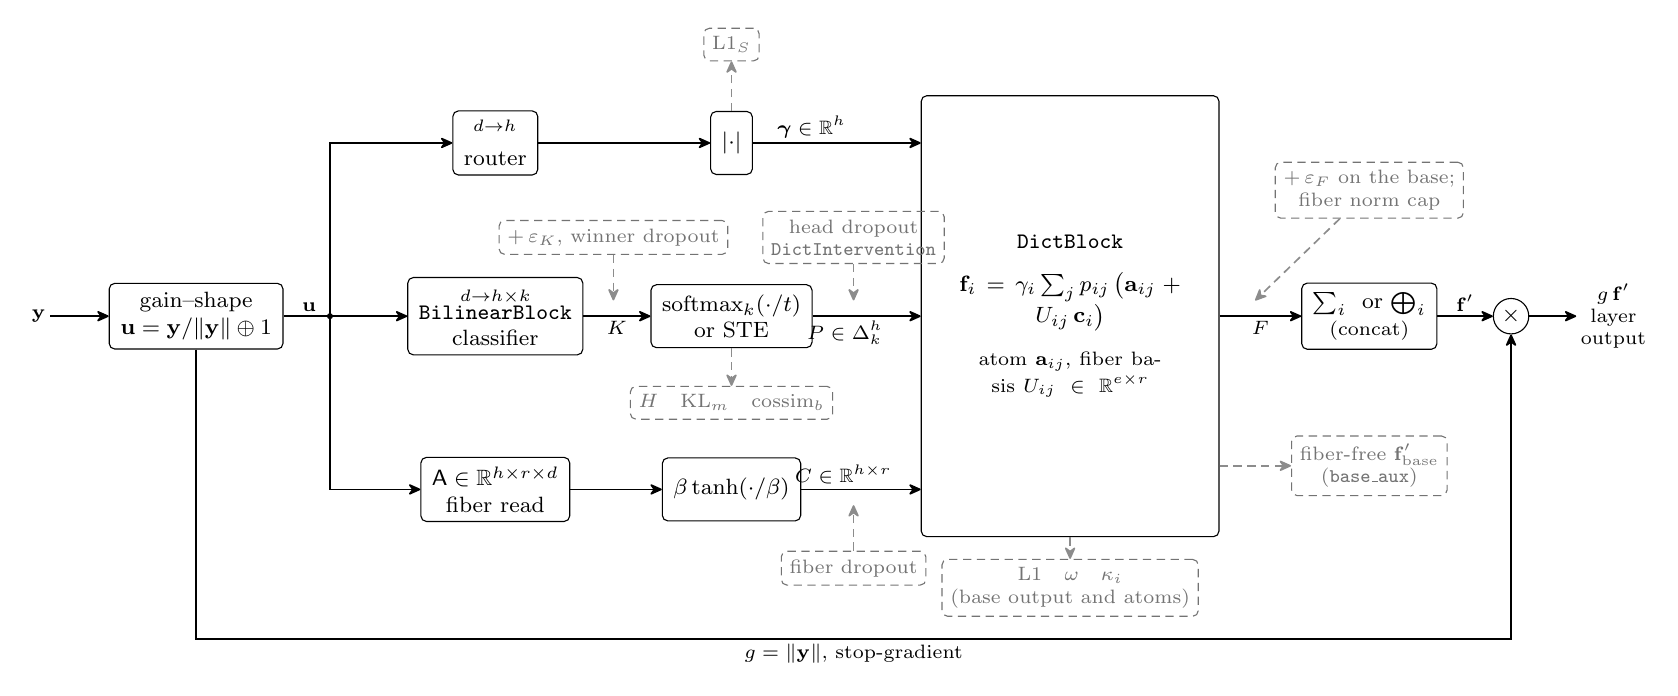
\begin{tikzpicture}[
    font=\footnotesize,
    >={Stealth[round,length=1.8mm,width=1.6mm]},
    blk/.style={draw, rounded corners=2pt, align=center,
                minimum height=8mm, inner xsep=4pt},
    hook/.style={draw, rounded corners=2pt, densely dashed, align=center,
                 inner sep=3pt, font=\scriptsize, black!55},
    mul/.style={draw, circle, minimum size=4.5mm, inner sep=0pt},
    lab/.style={inner sep=1.5pt, font=\scriptsize, align=center},
    sig/.style={->, semithick, align=center},
    aux/.style={->, densely dashed, semithick, black!45},
  ]

  %% ---- gain-shape split ------------------------------------------------
  \node[lab] (E)  at (-1.4,0) {$\mathbf{y}$};
  \node[blk] (GS) at ( 0.6,0) {gain--shape\\
                               $\mathbf{u}=\mathbf{y}/\lVert\mathbf{y}\rVert\oplus 1$};
  \draw[sig] (E) -- (GS);
  \coordinate (B) at (2.3,0);
  \draw[semithick] (GS.east) -- node[above,lab,pos=0.55]{$\mathbf{u}$} (B);
  \fill (B) circle (1.1pt);

  %% ---- three branches from u ---------------------------------------------
  % router: one non-negative scale per head
  \node[blk] (RT) at (4.4, 2.2) {$\bilinear^{d \to h}$\\ router};
  \node[blk] (AB) at (7.4, 2.2) {$\lvert\cdot\rvert$};
  % classifier: which entry, per head
  \node[blk] (CL) at (4.4, 0)   {$\bilinearblock^{d \to h \times k}$\\ classifier};
  \node[blk] (SM) at (7.4, 0)   {$\mathrm{softmax}_k(\cdot/t)$\\ or STE};
  % fiber read: r local coordinates per head
  \node[blk] (FR) at (4.4,-2.2) {$\mathsf{A} \in \mathbb{R}^{h \times r \times d}$\\ fiber read};
  \node[blk] (TB) at (7.4,-2.2) {$\beta\tanh(\cdot/\beta)$};

  \draw[sig] (B) |- (RT.west);
  \draw[sig] (B) -- (CL.west);
  \draw[sig] (B) |- (FR.west);
  \draw[sig] (RT) -- (AB);
  \draw[sig] (CL) -- node[below,lab]{$K$} (SM);
  \draw[sig] (FR) -- (TB);

  %% ---- the lookup ----------------------------------------------------------
  \node[blk, minimum height=5.6cm, text width=3.5cm] (DB) at (11.7,0)
    {$\dictblock$\\[6pt]
     $\mathbf{f}_i = \gamma_i \sum_{j} p_{ij}\,\big(\mathbf{a}_{ij}
            + U_{ij}\,\mathbf{c}_i\big)$\\[6pt]
     {\scriptsize atom $\mathbf{a}_{ij}$, fiber basis
      $U_{ij}\in\mathbb{R}^{e \times r}$}};

  \draw[sig] (AB) -- node[above,lab,pos=0.35]{$\boldsymbol{\gamma}\in\mathbb{R}^{h}$} (AB -| DB.west);
  \draw[sig] (SM) -- node[below,lab,pos=0.3]{$P\in\Delta_k^{h}$} (DB.west |- SM);
  \draw[sig] (TB) -- node[above,lab,pos=0.35]{$C\in\mathbb{R}^{h \times r}$} (TB -| DB.west);

  %% ---- combine heads, restore the gain --------------------------------------
  \node[blk] (CB) at (15.5,0) {$\sum_i$ \ or\ $\bigoplus_i$\\ {\scriptsize (concat)}};
  \node[mul] (MG) at (17.3,0) {$\times$};
  \node[lab] (F)  at (18.6,0) {$g\,\mathbf{f}'$\\ layer\\ output};
  \draw[sig] (DB.east |- CB) -- node[below,lab]{$F$} (CB);
  \draw[sig] (CB) -- node[above,lab]{$\mathbf{f}'$} (MG);
  \draw[sig] (MG) -- (F);
  \draw[sig] (GS.south) -- (0.6,-4.1) -| node[pos=0.25,below,lab]
       {$g=\lVert\mathbf{y}\rVert$, stop-gradient} (MG.south);

  %% ---- training-time hooks and the intervention interface (above) -------------
  \node[hook] (nk) at (5.9, 1.0) {$+\,\varepsilon_K$, winner dropout};
  \draw[aux] (nk) -- (5.9,0.2);
  \node[hook] (hd) at (8.95, 1.0) {head dropout\\ \texttt{DictIntervention}};
  \draw[aux] (hd) -- (8.95,0.2);
  \node[hook] (fd) at (8.95,-3.2) {fiber dropout};
  \draw[aux] (fd) -- (8.95,-2.4);
  \node[hook] (nf) at (15.5, 1.6) {$+\,\varepsilon_F$ on the base;\\
                                   fiber norm cap};
  \draw[aux] (nf) -- (14.05,0.2);

  %% ---- statistics (below) ------------------------------------------------------
  \node[hook] (sp) at (7.4,-1.1)
    {$H$\quad $\mathrm{KL}_m$\quad $\mathrm{cossim}_b$};
  \draw[aux] (SM.south) -- (sp);
  \node[hook] (ss) at (7.4, 3.45) {$\mathrm{L1}_S$};
  \draw[aux] (AB.north) -- (ss);
  \node[hook] (sf) at (11.7,-3.45)
    {$\mathrm{L1}$\quad $\omega$\quad $\kappa_i$\\ (base output and atoms)};
  \draw[aux] (DB.south) -- (sf);
  \node[hook] (ba) at (15.5,-1.9) {fiber-free $\mathbf{f}'_{\mathrm{base}}$\\
                                   (\texttt{base\_aux})};
  \draw[aux] (DB.east |- ba) -- (ba);

\end{tikzpicture}
}
\caption[\texttt{DictEnc} with router and fibers]{\textbf{\texttt{DictEnc}
	with router and fibers.} The gain--shape split hands the unit input
	$\mathbf{u}$ to three branches: the classifier (which entry, $P$),
	the router (how much, $\boldsymbol{\gamma}$, one non-negative scale per
	head) and the fiber read (where within the entry's fiber, $C$, $r$
	coordinates per head). They meet in the lookup
	(Equation~\ref{eq:fiber}); heads are summed, or concatenated under
	$\mathtt{ConcatDictBlock}$, and the result is scaled by the measured
	gain $g$. Dashed boxes above an arrow act on it during training;
	dashed boxes below are statistics, which describe the fiber-free
	base output. That output is also returned on its own for
	\texttt{base\_aux}.}
\label{fig:dictenc-full}
\end{figure}

\begin{figure}[tp]
\centering
% One head's geometry with a fiber, extending tikz/dict.tex: the head
% selects entry |d_{i2}|; its fiber is the plane U_{i2} spans at that entry,
% and the coordinates c_i place the output within it. The dashed circle is
% the norm cap (`fiber_eps`); the dotted ray is the radial variant, which
% only rescales the entry. Coordinates are precomputed (no calc library):
% d2 = (3.6, 3.2), basis columns u1 = (0.9, 0.25), u2 = (-0.2, 0.8).
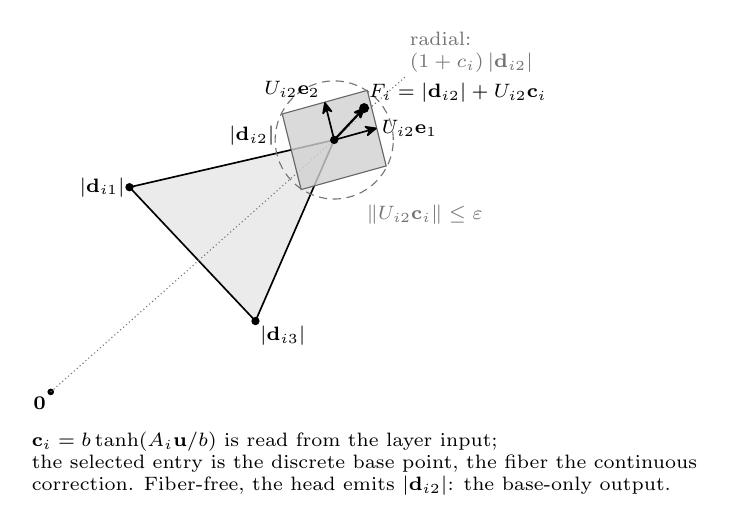
\begin{tikzpicture}[
    font=\footnotesize,
    >={Stealth[round,length=1.8mm,width=1.6mm]},
    lab/.style={inner sep=1.5pt, font=\scriptsize},
  ]
  %% ---- origin and the head's simplex ----------------------------------
  \fill (0,0) circle (1.2pt) node[below left,lab]{$\mathbf{0}$};
  \fill[black!8]   (1.0,2.6) -- (3.6,3.2) -- (2.6,0.9) -- cycle;
  \draw[semithick] (1.0,2.6) -- (3.6,3.2) -- (2.6,0.9) -- cycle;
  \fill (1.0,2.6) circle (1.5pt) node[left,lab]{$\lvert\mathbf{d}_{i1}\rvert$};
  \fill (2.6,0.9) circle (1.5pt) node[below right,lab]{$\lvert\mathbf{d}_{i3}\rvert$};

  %% ---- radial variant: a per-entry gain along the entry's own ray ------
  \draw[densely dotted, black!55] (0,0) -- (4.5,4.0)
    node[above right,lab,align=left]{radial:\\ $(1+c_i)\,\lvert\mathbf{d}_{i2}\rvert$};

  %% ---- the fiber at the selected entry ---------------------------------
  \fill[black!18, opacity=0.8]
    (4.02,3.83) -- (4.26,2.87) -- (3.18,2.57) -- (2.94,3.53) -- cycle;
  \draw[black!60]
    (4.02,3.83) -- (4.26,2.87) -- (3.18,2.57) -- (2.94,3.53) -- cycle;
  \draw[densely dashed, black!55] (3.6,3.2) circle (0.75);
  \node[lab, black!55] at (4.75,2.25) {$\lVert U_{i2}\mathbf{c}_i\rVert \le \varepsilon$};

  \draw[->, semithick] (3.6,3.2) -- (4.14,3.35)
    node[right,lab]{$U_{i2}\mathbf{e}_1$};
  \draw[->, semithick] (3.6,3.2) -- (3.48,3.68)
    node[above left,lab]{$U_{i2}\mathbf{e}_2$};

  \fill (3.6,3.2) circle (1.5pt);
  \node[lab, anchor=east] at (2.9,3.25) {$\lvert\mathbf{d}_{i2}\rvert$};

  %% ---- the output: base point plus its fiber offset ---------------------
  \draw[->, thick] (3.6,3.2) -- (3.98,3.605);
  \fill (3.98,3.605) circle (1.8pt);
  \node[lab, anchor=south west] at (3.98,3.62)
    {$F_i = \lvert\mathbf{d}_{i2}\rvert + U_{i2}\mathbf{c}_i$};

  %% ---- legend ------------------------------------------------------------
  \node[lab, anchor=north west, align=left] at (-0.3,-0.45)
    {$\mathbf{c}_i = b\tanh(A_i\mathbf{u}/b)$ is read from the layer input;\\
     the selected entry is the discrete base point, the fiber the continuous\\
     correction. Fiber-free, the head emits $\lvert\mathbf{d}_{i2}\rvert$:
     the base-only output.};
\end{tikzpicture}

\caption[Fiber geometry]{\textbf{Fiber geometry} for one head, extending
	Figure~\ref{fig:head-simplex}. The head selects the entry with atom
	$\mathbf{a}_{i2}$; its fiber is the plane spanned by
	$U_{i2}$ at that point, and the coordinates $\mathbf{c}_i$ place the
	output within it. The dashed circle is the per-head norm cap; the
	dotted ray is the radial variant, which moves the output only along
	the atom's own direction.}
\label{fig:fiber}
\end{figure}

\subsection{Training}
\label{sec:training}

\subsubsection{Embedding model}
\label{sec:sonar}
We embed texts using SONAR\cite{sonar}, a multimodal and
language-agnostic sentence embedding model. SONAR embeddings have
several desirable properties:
\begin{itemize}
	\item They correspond to entire texts rather than tokens.
	\item They are bidirectional.
	\item Language is encoded independently of text.
\end{itemize}
This allows us to validate steering fidelity against a ground truth.
Large Concept Models\cite{lcmteam2024largeconceptmodelslanguage}
generate directly in SONAR space, which makes it a natural substrate
for steering experiments.

\subsubsection{Loss function}
\label{sec:loss}
Reconstruction fidelity is trained with $\mathrm{MSE}$, where
$\mathbf{w} \in \mathbb{R}^d$ is a fixed per-dimension weight vector.

\begin{equation}
	\mathrm{MSE}(X,\hat{X}) := \frac{1}{bd}\sum^{b}_{n=1}\sum^{d}_{q=1}
	w_q\left(\hat{x}_{nq} - x_{nq}\right)^2
	\label{eq:mse}
\end{equation}

The total objective adds the ghost-gradient reconstruction and the
auxiliary statistics, each weighted by a scalar. Statistics are
\emph{summed} over the $l$ layers rather than averaged.

\begin{equation}
	L := \mathrm{MSE}(X,\hat{X})
	+ s_g\,\mathrm{MSE}(\hat{X}_g,\, X - \hat{X})
	+ \sum^{l-1}_{\ell=0}\mathbf{s}\cdot\boldsymbol{\psi}_\ell
	\label{eq:loss_total}
\end{equation}

Each layer contributes the statistics (Algorithms~\ref{alg:dictblock}
and~\ref{alg:dictenc})

\begin{equation}
	\boldsymbol{\psi}_\ell = \big[\,
	\mathrm{L1}_K \;\; \mathrm{L1} \;\; H \;\; \mathrm{cossim}_b \;\;
	\mathbb{E}_i\kappa_i \;\; \max_i \kappa_i \;\;
	\mathrm{KL}_m \;\; \mathrm{KL}_{\mathrm{pwak}} \;\; \mathrm{L2}_{\mathrm{pwak}}
	\;\; \mathrm{L1}_S \;\; \omega
	\,\big]^{\top}_\ell
	\label{eq:stats}
\end{equation}

where $\mathrm{L1}_K$ is the L1 of the classifier's gate, $\kappa_i$ the
mean within-head cosine between head $i$'s atoms,
$\mathrm{KL}_{\mathrm{pwak}}$ and $\mathrm{L2}_{\mathrm{pwak}}$ the two
partition-consensus statistics, and $\mathrm{L1}_S$ the router's L1. The
max of $\kappa_i$ is logged for a setpoint controller and never itself
penalized. Appendix~\ref{app:stats} gives the implementation's row
layout.

Each model's weights are in Appendix~\ref{app:configs}. The ghost path
is disabled throughout, since $\hat{X}_g$ fires only on features that
are exactly zero across the whole batch, which bilinear classifiers with
softmax selection and absolute-valued dictionaries never produce.

\begin{algorithm}[tp]
	\caption{$\ontologizer$ in training (\texttt{Ontologizer.withStats})
	and the loss it feeds (\texttt{Hyperparams.loss}), for the
	residual forward (\texttt{forward="resid"}) every configuration here
	uses. Without an encoder, $\mathrm{enc}$ is the identity; with direct
	atoms, $\mathrm{dec}$ is.}
	\label{alg:ontologizer}
	\DontPrintSemicolon

	\KwIn{batch $X \in \mathbb{R}^{b \times d}$}
	\KwData{encoder $\mathrm{enc}$; layers $\dictenc_1, \dots, \dictenc_l$
		(Algorithm~\ref{alg:dictenc}); decoder $\mathrm{dec}$
		(Eq.~\ref{eq:dec}); MSE weights $\mathbf{w}$; loss weights
		$\mathbf{s}$, $s_g$}
	\Hyper{input noise $\sigma_X$; deep supervision; \texttt{deepsup\_sg};
		\texttt{resid\_norm}, \texttt{resid\_const}, \texttt{resid\_gain}}
	\KwOut{loss $L$; per-layer statistics $\mathbf{m}_1, \dots,
		\mathbf{m}_l$}

	\Begin{
		$E \leftarrow \mathrm{enc}\big(\mathrm{noise}_X(X)\big)$
			\tcp*{Eq.~\ref{eq:noise_batchnorm}}
		$R \leftarrow \mathbf{0} \in \mathbb{R}^{b \times e}$;\quad
			$E \leftarrow E \oplus [1]$ \tcp*{if \texttt{resid\_const}}
		\For{$i \leftarrow 1$ \KwTo $l$}{
			$R_{\mathrm{prev}} \leftarrow R$\;
			$R, \mathsf{P}_i, \mathbf{m}_i \leftarrow \dictenc_i(R, E)$\;
			\If(\tcp*[f]{a decode per prefix}){deep supervision}{
				$\hat{X}_i \leftarrow \mathrm{dec}\big(R - R_{\mathrm{prev}}
					+ \mathrm{sg}[R_{\mathrm{prev}}]\big)$
					\tcp*{$\mathrm{dec}(R)$ without \texttt{deepsup\_sg}}
			}
			\If{$i < l$}{
				$Y \leftarrow \mathrm{sg}\big[X - \mathrm{dec}(R)\big]$
					\tcp*{Eq.~\ref{eq:L2}}
				$E \leftarrow Y / (\mathrm{L2}(Y) + \epsilon)$
					\tcp*{Eq.~\ref{eq:y_norm}; raw under
					\texttt{resid\_gain}}
				$E \leftarrow E \oplus [1]$
					\tcp*{if \texttt{resid\_const}}
			}
		}
		\lIf{not deep supervision}{$\hat{X}_l \leftarrow \mathrm{dec}(R)$}
		$\mathrm{MSE} \leftarrow \mathbb{E}_i\,
			\mathrm{MSE}_{\mathbf{w}}(X, \hat{X}_i)$
			\tcp*{Eq.~\ref{eq:mse}; each prefix weighted $1/l$}
		$L \leftarrow \mathrm{MSE} + s_g\,\mathrm{MSE}_g
			+ \mathbf{s} \cdot \sum_{i=1}^{l} \mathbf{m}_i$
			\tcp*{Eq.~\ref{eq:loss_total}; $\mathrm{MSE}_g = 0$ without
			ghosts}
		\Return{$L$, $(\mathbf{m}_i)_{i=1}^{l}$}\;
	}
\end{algorithm}


Reconstruction is trained with deep supervision:
$\mathrm{MSE}(X, \mathrm{dec}(R_\ell))$ is computed separately at
every layer and averaged, so each prefix carries weight $1/l$ and each
layer must explain what previous layers left
unexplained. The MSE is whitened: $\mathbf{w}$ in
Equation~\ref{eq:mse} is the per-dimension inverse variance, normalized
to mean one, the same whitening the evaluation applies. The
implementation applies $\sqrt{\mathbf{w}}$ to $X$ and
$\mathrm{dec}(R_\ell)$ before the squared error, which is equivalent.
Four statistics are active as loss terms in the reported models
(Figure~\ref{fig:dictenc}; Appendix~\ref{app:configs}):
between-sample similarity $\mathrm{cossim}_b$, computed from $P$
through the dictionary Gram so it measures feature-space similarity of
the per-head reconstructions, and which in practice also minimizes
per-sample entropy $H$; the batch-mean term $\mathrm{KL}_m$, anchoring
each head's mean
assignment vector to a uniform distribution so that a uniform code
corresponds to a maximally generic feature; an $\mathrm{L1}$ penalty on
features; and a between-head disjointness term, the support overlap
$\omega$, which measures the extent to which heads use nonoverlapping
coordinates of the dictionary space. Most reported models trained before
$\omega$ existed and used its predecessor (Appendix~\ref{app:stats}).
$\mathrm{L1}$ tends to fall under MSE alone; including it in the loss
speeds up convergence. Classification sharpness is controlled by the
temperature. Winner dropout and the noise terms
$\varepsilon_K$ and $\varepsilon_F$ regularize classifications and
features respectively.

\subsection{Evaluation}
Evaluation runs against $\topk$ SAEs trained on identical cached SONAR
embeddings under an identical whitened reconstruction objective. The
battery is deliberately SAEBench-style\cite{karvonen2025}: a
reconstruction-versus-capacity Pareto; categorical-form and
semantic-coherence tests of head structure; cross-model feature
splitting and seed stability; downstream text fidelity through the
paired M2M100 decoder; sparse language probing; shrinkage
decomposition; steering fidelity; and blinded auto-interpretability
scoring. A structural-ablation ladder of SAE variants, each adding one
Ontologizer-style commitment at a time, attributes effects to specific
structure. AxBench\cite{wu2025axbenchsteeringllmssimple} found that
simple supervised baselines beat SAEs at steering; the steering
comparison here is built to face that result.




\subsection{Data and objective}

\paragraph{Embedding space and data.}
All SONAR models are trained on a fixed cache of $N{=}4{,}000{,}000$
SONAR sentence embeddings ($d{=}1024$, unit-norm) computed from an
interleaved 86-language mC4 sample, with a language label sidecar. The
stream order is deterministic, so raw text is recoverable by row index
(verified against the language sidecar per row). The cloud is unit-normed
but not centred: $\lVert\mathbb{E}[x]\rVert = 0.564$, so it is a
spherical cap and $0.318$ of every squared norm is one shared direction.
It is dense without being isotropic --- effective dimension 108 of 1024
(participation ratio 268 on the whitened eval tail), yet 943 principal
components for 99\% of variance --- and samples average a pairwise cosine
of $0.31$. Section~\ref{sec:gpt2} additionally uses GPT-2~\cite{radford2019}
layer-8 residual-stream activations ($d{=}768$, harvested by
\texttt{encode\_acts.py}) as a substrate where sparse dictionary learning
is known to work.

\paragraph{Evaluation.}
All models minimize the whitened MSE of Equation~\ref{eq:mse}. We report
$\fvu$: whitened MSE divided by the whitened variance of a constant
predictor, on the final 32{,}768 cache rows. This tail is excluded from
SAE training and from the training of every straight-through arm.
\emph{Caveat: the softmax Ontologizers (\texttt{resid\_nc} and the
selection sweep) predate the holdout and trained on the full cache
including the tail, so their scores are in-sample; a fresh-encoded
evaluation set is future work.} Where activations are needed, Ontologizer
features are the flattened per-head classification probabilities
$P \in \Delta^{k}{}^{\,l\cdot h}$ at the run's final temperature (feature
$f = (l\cdot h + h_i)k + k_i$; fire threshold $2/k$), and SAE features are
latent activations (fire threshold $0$; grouped-softmax runs use the
above-uniform threshold $2/(m/G)$, matching the tag convention). Scoring a
softmax run at the default temperature $1.0$ rather than its annealed
$0.03$ puts a healthy checkpoint at $\fvu \approx 0.91$, which is
indistinguishable from a broken one; every number here uses the run's own
temperature.

\subsection{Models and baselines}

\paragraph{Softmax Ontologizers.}
The reference Ontologizer (\texttt{resid\_nc}, step 372{,}600) is the
architecture of Section~\ref{sec:arch}: $l{=}5$ residual layers, $h{=}32$
heads, $k{=}32$ entries per head, bilinear classifiers with residual
normalization and a constant input coordinate, deep supervision, and a
shared linear decoder from an $e{=}2048$ dictionary space; $\approx$23.1M
parameters and $l\cdot h\cdot k = 5{,}120$ dictionary entries. Layers
0--3 trained healthily (prefix $\fvu$ $0.129 \to 0.0051$); layer 4 froze
22/32 heads late in temperature annealing and is mildly harmful
(Section~\ref{sec:lastlayer} explains why). A later \emph{selection sweep}
holds that shape fixed and varies only the \texttt{DictBlock} selection
rule --- \texttt{top1}, \texttt{top2}, \texttt{top4}, \texttt{top8},
\texttt{top16}, \texttt{softmax} --- each with and without the
mean-entropy bonus raised to $s_{\mathrm{KL}_m}{=}3\times10^{-5}$
(\texttt{\_shm}), at 369{,}500 steps.

\paragraph{The straight-through arm.}
\texttt{train\_ste.py} imports \texttt{sonar.py}'s configuration and
overrides only \texttt{select="ste"}: the forward pass selects the argmax
one-hot, and the backward pass uses $\mathrm{softmax}(K/T)$ as its
surrogate. Its shape, calibration and initialization are described with
its results in Section~\ref{sec:ste}.

\paragraph{SAEs.}
SAEs follow Gao et al.~\cite{gao2024}: pre-activation
$\mathrm{relu}((x-b_{dec})W_{enc}+b_{enc})$ with top-$k$ selection,
unit-norm decoder rows, tied initialization, aux-$k$ dead-latent revival,
trained with Adam at $4\times10^{-4}$ for $\sim$144k steps at batch 4096
(converged; convergence is optimizer-step--limited, not epoch-limited, at
this batch size).

\paragraph{The structural-ablation ladder.}
To attribute differences to specific architectural commitments rather than
to whole architectures, we train SAE variants that each add one
Ontologizer-style constraint (all $m{=}5120$, same data and objective):

\begin{center}
\begin{tabular}{@{}llll@{}}
\toprule
rung & run & added structure & analogue \\
\midrule
1  & \texttt{k32} & none (top-$k{=}32$) & baseline \\
2a & \texttt{g160top1} & 160 groups, hard winner per group & heads (hard) \\
2b & \texttt{g160softmax} & 160 groups, softmax per group & heads (soft) \\
3  & \texttt{k32\_p5} & 5 nested prefix losses (matryoshka) & deepsup layers \\
--- & \texttt{k32\_bl} & bilinear encoder, $[x{-}b_{dec};1]$ factors & bilinear classifier \\
\bottomrule
\end{tabular}
\end{center}

Controls at width $m{=}11{,}264$ (parameter-matched to the Ontologizer):
\texttt{k32}, \texttt{k160} (coefficient-matched to one deviation per
head), and \texttt{k5120} (coefficient-matched to the full soft code; the
top-$k$ constraint never binds --- measured $L_0 \approx 1520$ --- so it is
effectively a dense ReLU autoencoder). A seed replica \texttt{k32\_s43}
supports stability analysis. The bilinear encoder's latents admit
closed-form ``eigenfeature'' analysis: each latent's symmetric form
$\mathrm{sym}(w_1 w_2^\top)$ is rank~2, with top-$|\lambda|$ eigenvector
$w_1/\|w_1\| \pm w_2/\|w_2\|$ (Pearce et al.~\cite{pearce2025}). Rung 2b
(\texttt{g160softmax}) is the load-bearing control under the steering
frame: it isolates the ``series of softmax classifiers'' idea from the
residual stack, bilinear classifiers, and shared dictionary.

\subsection{Evaluation protocols}

Each protocol is a standalone script sharing the eval split and activation
conventions; the root-level ones are unit-tested against planted-structure
synthetic data.

\paragraph{Capacity Pareto (\texttt{pareto.py}).}
Capacity is continuous coefficients transmitted per sample, plus index
bits. Ontologizer code points are \emph{top-$m$ deviation truncations}:
per head, keep the $m$ entries with largest $|p - \mathrm{origin}|$, pin
the rest to the origin distribution, renormalize. The origin is the
corpus-mean classification $\mathbb{E}[p]$ --- measured, not uniform: the
model output is jointly \emph{linear} in the flattened classifications
(zero residual seed, linear decoder), so $\mathrm{decode}(\mathbb{E}[p]) =
\mathbb{E}[Y]$, which decodes to the corpus-mean generic text, while the
uniform code lands off-manifold (cosine $0.067$ to $\mathbb{E}[X]$) ---
despite $\mathrm{KL}_m$ being included in the loss precisely to make the
uniform code the generic one (Section~\ref{sec:labels}). Endpoints:
$m{=}0$ (input-independent origin), $m{=}k$ (exact soft model), and
end-to-end argmax (``hard''). An alternative head-level code mean-ablates
all but the $m$ lowest-entropy heads per layer. SAE points use measured
eval $L_0$. A hard code's index bits are $l\cdot h\log_2 k$; we compare
each against the reverse water-filling bound~\cite{cover2006} on the
whitened eval-tail covariance, the best distortion \emph{any} code of
that rate can reach under a Gaussian model.

\paragraph{Categorical form (\texttt{headstruct.py}).}
An Ontologizer head is exhaustive (always fires) and exclusive (one
winner). We test whether SAE latents form such units: discovery clusters
latents by \emph{paradigmatic} affinity --- similar co-fire profiles with
the rest of the dictionary $\times$ anti-correlation with each other
(PMI${}<1$) --- under a group-size cap, on one half of the rows; scoring
on the held-out half computes per-group exhaustiveness $P(\text{any
fires})$, exclusivity $\mathbb{E}[\#\text{firing} \mid \geq 1]$, and the
CV of summed activation, against size-matched random partitions of the
live-latent pool. Head-like structure requires exhaustiveness \emph{above}
null with exclusivity \emph{below} null; topical co-firing clusters show
the opposite signature. \texttt{--trained-groups} scores a grouped run's
own partition.

\paragraph{Semantic coherence vs.\ contrast (\texttt{headcoh.py}).}
The complement to categorical form: do a head's entries \emph{mean}
similar things, or do they form a contrast set? Every entry has an exact
decode direction in SONAR output space --- for the Ontologizer, the rows
of the linear map $G$ with $Y = P_{\text{flat}}G$; for SAEs, decoder rows
--- and SONAR space is a semantic sentence space, so within-head direction
similarity is semantic similarity of what entries decode to. Per head we
report mean pairwise cosine and top-singular-value energy fraction,
$z$-scored against size-matched random subsets of the same pool (same
layer for Ontologizer heads); as a metric-hygiene control the same
statistics are recomputed under the training objective's inverse-variance
inner product (\texttt{--metric whitened}). $z \gg 0$ means a head clusters
semantically; $z \ll 0$ means its entries repel --- the signature of a
\emph{contrastive classifier}, whose class decoders are pushed apart. A
second view SONAR-encodes auto-interp description texts and tests pooled
within-head similarity against a label-permutation null.
\texttt{--assignment} scores discovered (post-hoc) groups.

\paragraph{Feature splitting and seed stability (\texttt{splitting.py},
\texttt{partition.py}).}
For models $A$ (coarse) and $B$ (fine) on shared rows, each $B$-latent is
classified per $A$-parent by two-way firing containment at threshold
$\tau$: a \emph{child} satisfies $P(A_i \mid B_j) \geq \tau$,
$P(B_j \mid A_i) < \tau$; a \emph{match} satisfies both. Splits
($\geq 2$ children) are scored by union coverage of the parent's firing
set and pairwise child overlap. Decoder geometry adds absorption
candidates (decoder-cosine twins that do not co-fire) and each model's
nearest-neighbour decoder-cosine distribution vs.\ a random baseline. For
two same-architecture runs differing only in seed, the match fractions
are the reproducible-feature fractions. For hard-code Ontologizers,
\texttt{partition.py} matches heads across runs by the NMI of their
partitions (Hungarian assignment within layer) against a shuffled null,
and the same-run comparison against an earlier checkpoint serves as the
positive control.

\paragraph{Text fidelity (\texttt{textfid.py}).}
The ``loss recovered'' analogue: decode $x$ and $\mathrm{recon}(x)$
through M2M100 (forced \texttt{eng\_Latn}, both rescaled to the reference
SONAR norm, so the metric sees direction error) and report
chrF~\cite{popovic-2015-chrf} and exact-match between the decodes, plus the
decoder's teacher-forced per-token NLL of the \emph{original's} decode
under the original (ceiling), the reconstruction, and the corpus-mean
embedding (floor --- which decodes to the generic text). Under the
steering frame this doubles as the collateral ceiling: a code that cannot
preserve text cannot steer text with low collateral.

\paragraph{Language probing (\texttt{langprobe.py}, \texttt{headlang.py},
\texttt{headscript.py}).}
SAEBench-style $k$-sparse probing with the free 86-language labels: top
latents per language by two-sample $t$-statistic on training rows;
held-out one-vs-rest F1 at $k{=}1$ (single latent, fitted threshold),
$k{=}4,16$ (logistic probes), and a dense probe on the raw embedding as
ceiling. Macro-F1 over languages. \emph{Frame caveat: this measures
whether a factor lives in individual latent magnitudes. A classifier head
carries its factor in its assignment (partition), which single-latent
probes cannot see.} \texttt{headlang.py} is the matching instrument: per
head, the NMI between its partition and the label, null-corrected by a
label shuffle, plus a held-out probe on the best $m$ heads' one-hot
codes against a dense ridge ceiling. NMI here normalizes by the
arithmetic mean of the two entropies, so its attainable maximum is
$2\min(H_h,H_\ell)/(H_h+H_\ell)$ --- $0.875$ for a 5-bit head against the
6.43-bit language label. \texttt{headscript.py} repeats this for script
and scores per-label tag cells and cross-head conjunctions;
\texttt{headeta.py} measures each partition's $\eta^2$ in embedding
space, corrected by the $(g-1)/(n-1)$ a random $g$-way partition scores.

\paragraph{Shrinkage (\texttt{refit.py}).}
Gao-style refinement: freeze each sample's support, solve the whitened
least-squares coefficients (masked normal equations; silent group slots
forced to zero), and compare $\fvu$. Raw$-$refit is magnitude (shrinkage)
error; refit is selection error. The Ontologizer shares the machinery via
its exact linearity $Y = P_{\text{flat}} G$, with $G$ measured by decoding
one-hot constant codes; its supports are the top-$m$ deviation entries.
Points with support $\geq d$ are excluded (underdetermined). Note the raw
convention: \texttt{refit.py} truncates the soft forward's $P$
(non-adaptive), whereas \texttt{pareto.py} truncates inside the forward,
letting later layers reclassify against the truncated prefix residual.

\paragraph{Steering fidelity in text (\texttt{steerfid.py}).}
Unit-normalized native steering directions --- SAE decoder rows, bilinear
eigenfeatures, or the Ontologizer's \texttt{withArgs} set-intervention
delta --- applied at matched embedding magnitudes. Effect is cycle
consistency: the steered decode is re-encoded through SONAR and the target
feature's activation gain is normalized by its firing-conditioned
quantiles, with the baseline taken from the \emph{cycled} base decode so
both sides share roundtrip degradation. Collateral is $1 - \mathrm{chrF}$
against the base decode. Random unit directions give the control curve,
and \emph{net} effect is feature effect minus that control.

\paragraph{Steering fidelity in embedding space (\texttt{steerembed.py}).}
Drops the text round trip and asks the causal question directly: move
the input along a direction, re-run the model, and record whether the
intended entry is now selected (\emph{realization}) and what fraction of
the \emph{other} heads changed their selection (\emph{collateral}).
Directions: \texttt{decode} (the decode delta of forcing the entry),
\texttt{grad} (the gradient of the target logit), \texttt{margin} (the
gradient of the target's margin over the head's current winner),
\texttt{adjoint} (the bilinear classifier's top eigenvector via
\texttt{BilinearBlock.rev}), and \texttt{random}. 64 entries, 32 held-out
rows each, steered only where the entry was not already selected.

\paragraph{Intervention composition (\texttt{compose.py}).}
Treating heads as candidate causal variables: for pairs of forced
assignments $(l_1,h_1){\to}k_1$, $(l_2,h_2){\to}k_2$ (8 random heads per
layer, one random entry each; all same-layer pairs plus 60 cross-layer
pairs), compare the joint intervention's decode delta $D_{12}$ against
the sum $D_1{+}D_2$ of the single-intervention deltas on 512 held-out
rows: median per-row cosine and relative error
$\|D_{12}-(D_1{+}D_2)\|/\|D_1{+}D_2\|$, raw and whitened. Because the
decode is exactly linear in the flattened classification, final-layer
pairs compose exactly by construction; that stratum doubles as the
measured numerical floor (the $\|R\|{\approx}31 \to \|Y\|{\approx}1$
decoder cancellation amplifies float32 rounding to ${\sim}0.02$ relative
error between differently-compiled variants --- verified exact in
float64). All other non-additivity is downstream reclassification:
later layers re-reading the intervened residual.

\paragraph{Auto-interpretability (\texttt{autointerp.py}).}
Four stages: harvest (top-activating rows, negatives, frequency-stratified
feature selection, parameter-based decode embeddings), texts
(deterministic mC4 stream replay recovers text by row index, verified
against the language sidecar), describe, and score. Description modes:
\texttt{params}, the M2M100 decode of a parameter-derived embedding (for
tags, the $\mathbb{E}[p]$-origin code with one head forced one-hot; for
SAE latents, $b_{dec} + \alpha W_{dec,j}$); \texttt{pdev}, the same decode
with the pure-origin decode subtracted; \texttt{eig}, the bilinear
eigenfeature decode; \texttt{acts}, an LLM summary of top-activating
snippets; and \texttt{cacts}, a \emph{contrastive} summary --- the judge
sees top snippets next to random corpus draws and must name what
distinguishes them, blocking the degenerate corpus-level answer that
plain summaries invite on noisy multilingual web text. Scoring is blinded
detection over held-out positives and negatives, identical for all
modes; per-feature F1, to be read against the always-match null of
$\mathrm{F1} \approx 0.67$ on balanced items. The judge is Haiku
(\texttt{claude-haiku-4-5}) via the Anthropic Messages API, rate-metered,
with bounded reply length; failed judgements are never recorded (an
earlier outage mode scored empty replies as $\mathrm{F1}=0$). Six models:
the Ontologizer, rungs \texttt{k32}/\texttt{k32\_bl}/\texttt{g160top1}/%
\texttt{g160softmax}, and the dense control \texttt{k5120}.

\paragraph{Diagnostic scripts (\texttt{experiments/ste-arm/}).}
The straight-through and geometry results rest on further single-purpose
instruments, described where used: \texttt{inputgeom.py} (geometry of the
vector each classifier sees), \texttt{blendablate.py} (severing the
pairing between a layer's input and the sample's own earlier
reconstruction), \texttt{gainablate.py} (the norm side-channel),
\texttt{dictgeom.py} (row collinearity and effective rank read from the
weights), \texttt{lastlayer.py} (final-layer ablations against the
deep-supervision prefixes), \texttt{decodehead.py} (decoding a head's
entries as deviations from its mean), and \texttt{embedgeom.py} (SONAR
cloud geometry).

\section{Results: the softmax Ontologizer against SAEs}

\subsection{The price of structure: reconstruction--capacity Pareto}
\label{sec:pareto}

\begin{table}[h]\centering\small
\begin{tabular}{@{}lrrr@{}}
\toprule
point & coeffs & index bits & $\fvu$ \\
\midrule
onto $m{=}0$ ($\mathbb{E}[p]$ origin) & 0 & 0 & 1.001 \\
onto hard (argmax)                  & 0 & 800 & 17.34 \\
\emph{rate floor at 800 bits}       & 0 & 800 & \emph{0.226} \\
sae k32 tier ($m{=}5120/11264$, incl.\ p5, s43) & 32 & $\sim$400 & 0.494--0.509 \\
sae k32 bilinear                    & 32 & 394 & 0.602 \\
onto dev $m{=}1$                    & 160 & 800 & 0.677 \\
sae g160top1                        & 160 & 1972 & 0.274 \\
sae k160 ($m{=}11264$)              & 160 & 2154 & 0.258 \\
onto dev $m{=}2$                    & 320 & 1600 & 0.497 \\
onto dev $m{=}4$                    & 640 & 3200 & 0.289 \\
onto dev $m{=}8$                    & 1280 & 6400 & 0.094 \\
sae k5120 ($m{=}11264$, $L_0{\approx}1520$) & 1520 & 20455 & \textbf{0.00011} \\
onto dev $m{=}16$                   & 2560 & 12800 & 0.0082 \\
sae g160softmax                     & 5120 & 0 & \textbf{0.00436} \\
onto soft ($m{=}32$)                & 5120 & 0 & 0.00538 \\
\bottomrule
\end{tabular}
\caption{Reconstruction vs.\ code capacity for \texttt{resid\_nc}, shared
eval tail. The plain-SAE frontier dominates the Ontologizer's deviation
code at every measured capacity; the gap is the price paid for
contrast-set structure in a soft code.}
\end{table}

Findings. (1) At matched $\fvu \approx 0.49$, the SAE transmits 32
coefficients where the Ontologizer needs 320 (a 10$\times$
coefficient-efficiency gap), with the caveat that top-$m$ points are
post-hoc truncations of a model never trained to truncate. (2) The
Ontologizer's granularity floor (one deviation per head, 160 coefficients,
$\fvu\,0.677$) is worse than the SAE's 32-coefficient point --- the very
sparse regime is structurally closed to it. (3) The parameter- and
coefficient-matched dense control (\texttt{k5120}) reaches
$\fvu\,1.1\times10^{-4}$ with $3.4\times$ fewer active coefficients than
the soft Ontologizer: unstructured reconstruction is $\sim$50$\times$
better at matched budgets. (4) Head-level codes (mean-ablate all but the
$m$ lowest-entropy heads) are far weaker than deviation codes at matched
coefficients (heads $8/32$: $0.50$ vs.\ dev $m{=}8$: $0.094$):
reconstruction information is spread near-evenly across all 160 heads ---
under the classifier reading, every head's assignment carries signal for
every input, which is what a MoEfied code should look like, and why
per-sample head \emph{confidence} does not localize reconstruction.
(5) Uniform-origin truncation is strictly worse than
$\mathbb{E}[p]$-origin (dev $m{=}1$: $0.98$ vs.\ $0.68$): the measured
mean classification, not uniform, is the code's true origin; neutral
ablations and steering baselines should pin to it. (6) The soft model's
own discrete reading is not a code at all. The argmax row is 77$\times$
above the best distortion \emph{any} 800-bit code can reach ($0.226$),
and on the selection sweep's \texttt{softmax\_shm} run the gap is nine
orders of magnitude (argmax $\fvu$ $8.7\times10^6$ against $0.0007$ soft).
The tags that \texttt{decode.py}'s interventions and
\texttt{decode\_tags.py} read are therefore not what carries a softmax
model's embedding --- the motivation for Section~\ref{sec:ste}. Even a
perfect 800-bit code would sit near $\fvu\,0.23$: the live head count is
too small for a discrete ontology to be possible at all.

\subsection{Structure decomposition (the ladder)}

\begin{table}[h]\centering\small
\begin{tabular}{@{}lrrl@{}}
\toprule
rung & $\fvu$ & $L_0$ & note \\
\midrule
k32 baseline    & 0.499 & 32   & 0 dead \\
g160top1        & 0.274 & 160  & 1434/5120 dead (28\%) \\
g160softmax     & \textbf{0.0044} & 5120 & beats \texttt{resid\_nc} (0.0054) \\
k32\_p5         & 0.509 & 32   & deepsup tax $\sim$2\% \\
k32\_bl         & 0.602 & 32   & 1848/5120 dead (36\%) \\
\bottomrule
\end{tabular}
\caption{Converged structural rungs, $m{=}5120$, 144.3k steps each.}
\end{table}

The grouped-simplex code constraint alone costs $\sim$30$\times$ vs.\ the
unstructured dense control ($0.0044$ vs.\ $1.1\times10^{-4}$); against
\texttt{resid\_nc}, everything the Ontologizer adds beyond rung 2b ---
bilinear classifiers, five residual layers, the shared 2048-d dictionary
space --- adds \emph{nothing} to reconstruction (slightly negative), at
$2.2\times$ the parameters. That verdict is specific to the reference
checkpoint: the selection sweep's \texttt{softmax\_shm} run, identical in
shape, reaches $0.0007$ on the same tail (in-sample, like
\texttt{resid\_nc}), six times below \texttt{g160softmax}. The stack can
therefore beat its single-layer rival on reconstruction; whether it does
so out of sample is open. Hard-per-group selection costs only $\sim$6\%
over an unstructured code of equal sparsity (\texttt{g160top1} 0.274
vs.\ \texttt{k160} 0.258), which also shows the Ontologizer's
catastrophic argmax code ($\fvu\,17.3$; one-hot selection inflates output
norm $3.7\times$ because winner entries carry $\sim$4$\times$ the
soft-mixture norm) is a training artifact, not intrinsic to discrete head
codes --- Section~\ref{sec:ste} confirms this from the Ontologizer side.
Nested prefix losses are nearly free. The bilinear encoder costs
$\sim$20\% $\fvu$ and kills a third of the dictionary. Under the steering
frame, the ladder's implication is pointed: \emph{the classifier-forming
ingredient is grouped softmax itself}; whether the full stack earns its
extra cost must be decided by task naturalness and steering quality, not
reconstruction.

\subsection{Categorical form}

At 1M rows with split-half scoring and 20 size-matched nulls:
\texttt{g160top1}'s trained partition is \emph{perfectly} head-like
(exhaustiveness $1.0000$ vs.\ null $0.64$; exclusivity $1.0000$ vs.\
$1.51$; sum-CV $0.25$ vs.\ $1.03$). Discovery on every unstructured run
(\texttt{m11264\_k32}, \texttt{m5120\_k32}, \texttt{k32\_p5},
\texttt{m11264\_k160}) finds the \emph{opposite} signature ---
exhaustiveness below null ($z$ from $-30$ to $-50$), exclusivity above
($z$ $+13$ to $+31$): spontaneous SAE group structure consists of
co-firing topical clusters, not categorical slots, even when the affinity
explicitly selects for anti-correlated same-context pairs. And
\texttt{g160softmax} never fires distinctly at all: no coefficient ever
exceeds $2/32$ on any test row --- soft grouped codes converge to dense
near-uniform mixtures, exactly as the Ontologizer's soft code does
($\mathbb{E}[p]$ sits $0.06$--$0.16$ bits from uniform in healthy layers;
matching soft reconstruction requires $\sim$16 of 32 deviations per head).
\textbf{Categorical structure exists precisely when trained in as hard
selection, never emerges from softmax competition under a reconstruction
objective, and costs $\sim$60$\times$ in $\fvu$ (0.274 vs.\ 0.0044)
at the SAE's 160 heads.} For steering this means the \emph{soft}
architectures' classifier reading must be cashed out in deviations around
$\mathbb{E}[p]$, not in discrete winners --- or the selection must be
made hard during training, which Section~\ref{sec:ste} does at a far
smaller cost once the head count is raised.

\subsection{Semantic coherence: heads are contrast sets}
\label{sec:prelim-orth}

\begin{table}[h]\centering\small
\begin{tabular}{@{}lrrrr@{}}
\toprule
grouping & groups & mean $z_{\cos}$ & frac $z{>}2$ & frac $z{<}{-}2$ \\
\midrule
g160top1 (trained, hard)      & 160 & $+161.3$ & 1.00 & 0.00 \\
k32 discovered (\texttt{m11264}) & 359 & $+1.7$ & 0.36 & 0.02 \\
onto heads (trained, soft)    & 160 & $-17.6$ & 0.04 & \textbf{0.96} \\
g160softmax (trained, soft)   & 160 & $-14.7$ & 0.00 & \textbf{1.00} \\
\bottomrule
\end{tabular}
\caption{Within-head decode-direction coherence vs.\ size-matched
same-pool nulls (\texttt{headcoh.py}, $n_{\text{null}}{=}500$).}
\end{table}

This is the sharpest dissociation in the battery, and the one the
steering goal predicts. Hard-trained groups are hugely \emph{coherent}
(every \texttt{g160top1} group far above null: winner-take-all carves the
data so each group's entries tile one decoder cluster --- fine-grained
substitutions within a region). Post-hoc co-fire clusters are mildly
coherent (topical). But both soft classifier architectures are
\emph{anti-coherent}: in 96--100\% of heads, the entries' decode
directions are \emph{more mutually dissimilar than random same-pool
sets}. Softmax competition pushes a head's class decoders apart ---
within-head entries are well-separated alternatives, i.e.\ heads function
as \emph{contrastive classifiers}, and within-head swaps are large, clean
moves along the head's own dimension. Notably the signature is shared by
the Ontologizer and single-layer \texttt{g160softmax} with near-identical
strength. The choice of inner product is not doing the work: recomputed
under the whitened metric the training objective actually optimizes, the
repulsion \emph{strengthens} for the Ontologizer (mean $z_{\cos}$
$-24.4$ vs.\ $-17.6$ raw; frac $z{<}{-}2$ unchanged at $0.96$) and is
essentially unchanged for \texttt{g160softmax} ($-14.7$) and
\texttt{g160top1} ($+179.3$ vs.\ $+161.3$).

The hard-code Ontologizer agrees from the weights side. Its within-head
row cosine, decoded into output space, is $0.023$ at layer 0 and $-0.015$
to $-0.020$ at layers 1--4: a head's entries are essentially orthogonal,
and slightly repelling, in the space that matters. The same statistic read
in the $e$-dimensional dictionary space instead reads $0.12$--$0.29$; that
reading is dominated by the decoder's null space and should not be used
(Section~\ref{sec:rowcos}). Of the two orthogonalities in
Section~\ref{sec:disjoint}, then, the within-head one is measured and
holds in both code types.

Two \texttt{resid\_nc} outlier heads (layer-2 h25, $z{+}346$; layer-3
h28, $z{+}280$; the next candidates sit in the partially frozen layer 4)
cluster instead of contrasting --- their sampled entries also decode to
generic text, so we suspect partial head collapse (entries never
differentiated), not semantic coherence; targeted inspection pending.
The description-text view was uninformative on plain summaries
($\sim$77\% generic corpus descriptions for tags, 49\% for k32 latents,
inflating the permutation null: pooled $z=-0.25$); re-run on the
contrastive \texttt{cacts} descriptions it acquires signal. Within-head
description similarity clears the head-label permutation null for
\texttt{g160top1} ($z{=}{+}2.42$, 62 within-head pairs), is marginal for
Ontologizer heads ($z{=}{+}1.92$, 155 pairs), and is absent for
\texttt{g160softmax} ($z{=}{+}0.79$, 217 pairs). Read against the
geometry this is the pattern ``alternative values of one shared
dimension'' predicts: Ontologizer entries' decode \emph{directions}
repel while their described \emph{contents} weakly cohere. It is also
the first instrument in the battery to separate the Ontologizer from
its single-layer soft rival, whose head contents show no description
coherence at all --- suggestive rather than significant at this
coverage (one global $z$ per model over the campaign's sampled
features).

\subsection{Feature reliability}

Seed stability (\texttt{k32} vs.\ \texttt{k32\_s43}; identical
architecture and data, $\fvu$ 0.4994 vs.\ 0.4967): matched-feature
fractions are \textbf{0.31 / 0.24 / 0.15 / 0.03} at
$\tau = 0.3/0.5/0.7/0.9$. Roughly three quarters of individual features
are not reproducible across initializations at moderate containment.
Cross-width splitting (\texttt{k32} $\to$ \texttt{m11264\_k32}): 190 of
5114 live parents split at $\tau{=}0.7$ (median 3 children; union
coverage 0.37; child overlap 0.42), with 441 absorption candidates and a
heavy nearest-neighbour decoder-cosine tail (p50 0.234 vs.\ random
0.119): splitting is real but is not the dominant organization; topical
co-firing is. For a steering generator the unit that must reproduce is
the head's partition rather than the individual feature vector;
Section~\ref{sec:seeds} measures that on the hard-code Ontologizer and
finds it reproduces far \emph{worse} than SAE features do.

\subsection{Text-space fidelity (collateral ceiling)}

\begin{table}[h]\centering\small
\begin{tabular}{@{}lrrr@{}}
\toprule
model & chrF & exact & NLL (ceil.\ $\approx$1.56--1.63, floor $\approx$3.8) \\
\midrule
corpus-mean floor & $\approx$0.20 & 0 & 3.60--3.89 \\
k32 tier (incl.\ p5, m11264) & 0.23 & 0.00 & 3.00--3.08 \\
k32\_bl          & 0.21 & 0.00 & 3.19 \\
k160 / g160top1  & 0.28--0.29 & 0.00 & 2.34--2.37 \\
onto soft        & 0.538 & 0.090 & 1.658 (gap 0.026) \\
g160softmax      & 0.592 & 0.119 & 1.563 (gap 0.007) \\
k5120            & 0.856 & 0.592 & 1.587 (gap 0.000) \\
\bottomrule
\end{tabular}
\caption{Downstream text fidelity, 512 tail rows, forced English decodes.}
\end{table}

The FVU--text mapping is sharply nonlinear: $\fvu \approx 0.5$ decodes to
same-topic-different-facts text barely above the generic floor, while the
Ontologizer's soft code and \texttt{g160softmax} are near the likelihood
ceiling --- almost all decodable content survives. Across the eleven
Ontologizer runs with both numbers (the selection sweep and the
straight-through arms; Table~\ref{tab:steerfid}), ``loss recovered'' is a
monotone function of $\fvu$ (rank correlation essentially $-1$), so text
fidelity is a check that the whitened objective transports to text, not
an independent axis --- and it does. This matters doubly under the
steering frame: a steering primitive that routes through a code which
cannot preserve text (the entire $k{\leq}160$ sparse tier) starts from
$\sim$0.75 collateral before any intervention, whereas the dense-mixture
classifier codes start near zero.

\subsection{Concept (language) localization}

\begin{table}[h]\centering\small
\begin{tabular}{@{}lrrrr@{}}
\toprule
model & F1@1 & F1@4 & F1@16 & dense \\
\midrule
k160          & \textbf{0.119} & 0.393 & \textbf{0.473} & 0.676 \\
k32 ($m{=}5120$) & 0.089 & 0.347 & 0.465 & 0.676 \\
m11264\_k32   & 0.078 & 0.364 & 0.471 & 0.676 \\
k32\_bl       & 0.084 & 0.228 & 0.368 & 0.676 \\
g160softmax   & 0.068 & 0.162 & 0.328 & 0.676 \\
g160top1      & 0.066 & 0.200 & 0.302 & 0.676 \\
k32\_p5       & 0.061 & 0.322 & 0.454 & 0.676 \\
k5120         & 0.064 & 0.130 & 0.237 & 0.676 \\
onto (tags)   & 0.022 & 0.021 & 0.117 & 0.677 \\
\bottomrule
\end{tabular}
\caption{Macro one-vs-rest F1 over 86 languages, held-out tail.}
\end{table}

Language remains distributed in every model (best single-latent macro-F1
0.119 vs.\ dense ceiling 0.676; script-distinctive languages such as
Chinese reach $\sim$0.98 from one latent, same-script families smear),
and localization \emph{anticorrelates} with reconstruction across the
family. The Ontologizer's tag probabilities are decisively the worst
localizers (F1@1 $=0.022$). Read on SAE terms this is an indictment; read
on classifier terms it is expected: a head encodes a factor in its
\emph{assignment}, not in any single tag's magnitude, and partition-level
analysis of \texttt{resid\_nc} found layer-1 heads whose partitions carry
script/family mutual information, one of which ((L1,h8,k17)) was causally
verified to force Burmese output. The partition-level instrument
(\texttt{headlang.py}) was later run on a config-matched softmax
reference and on the hard-code arms (Section~\ref{sec:lang}): the softmax
reference's best head reaches a null-corrected NMI of only $0.043$, a
sixth of the hard code's. Language factors are carried by a \emph{few}
heads' partitions, weakly, and most heads classify something else.

\subsection{Shrinkage decomposition}

Top-$k$ SAEs have small magnitude error (share of raw $\fvu$ removed by
support-frozen least squares: 2.2--2.4\% for k32 variants, 8.5\% for
k160, 0.6\% bilinear, 1.9\% p5); \texttt{g160top1} is essentially
perfectly calibrated (0.3\%) --- its reconstruction deficit is pure
selection. The Ontologizer's truncated deviation codes are
magnitude-heavy: 16\% at $m{=}1$, 33\% at $m{=}2$, i.e.\ the
pin-and-renormalize convention mis-scales what it keeps (supports of
$\geq d$ coefficients are excluded as underdetermined). Separately, the
gap between non-adaptive truncation (freeze soft $P$, truncate, decode
linearly) and in-forward truncation (later layers reclassify against the
truncated prefix residual) is large --- $0.268$ vs.\ $0.094$ at $m{=}8$:
downstream layer compensation is worth $\sim$3$\times$ under truncation.
This was the first quantified reconstruction credit for the residual
stack (Section~\ref{sec:depth} measures a larger one), and it is
steering-relevant: the stack actively re-routes around code edits, which
cuts both ways --- robustness to small interventions, and, as
Section~\ref{sec:entangle} shows, widespread collateral.

\subsection{Steering fidelity}
\label{sec:steer}

\paragraph{In text.}
On the SAE side only a smoke-scale run exists (k32, 3 features):
cycle-consistency effect rises with magnitude (1.2 $\to$ 1.8 over
magnitudes 0.5 $\to$ 1.0 relative to the unit input norm; hit rate 0.67
$\to$ 0.89), while collateral at these magnitudes ($\approx$0.75) is near
the random-direction control. Across the Ontologizer selection sweep and
the straight-through arm, at 64 features per run:

\begin{table}[h]\centering\small
\begin{tabular}{@{}lrrrrrrrr@{}}
\toprule
run & $\fvu$ & chrF & loss rec. & net @0.25 & @0.5 & @1.0 & hit @1.0 & rand.\ hit \\
\midrule
top8          & 0.0370 & --- & 0.940 & 0.131 & 0.303 & \textbf{0.580} & 0.713 & 0.277 \\
top2          & 0.3516 & 0.248 & 0.532 & 0.125 & 0.289 & 0.474 & 0.564 & 0.217 \\
top16         & 0.0052 & --- & --- & 0.065 & 0.119 & 0.243 & 0.313 & 0.139 \\
top8\_shm     & 0.0287 & 0.416 & 0.956 & 0.072 & 0.096 & 0.193 & 0.291 & 0.142 \\
softmax\_shm  & 0.0007 & 0.694 & 0.998 & 0.032 & 0.072 & 0.146 & 0.150 & 0.064 \\
top2\_shm     & 0.1911 & 0.303 & 0.738 & 0.022 & 0.070 & 0.141 & 0.154 & 0.041 \\
top4\_shm     & 0.0761 & 0.360 & 0.897 & --- & --- & --- & --- & --- \\
\texttt{ste\_h76} & 0.2293 & 0.282 & 0.702 & 0.072 & 0.096 & 0.107 & 0.068 & 0.062 \\
top1          & 0.7190 & 0.180 & 0.123 & 0.011 & 0.026 & 0.048 & 0.069 & 0.020 \\
\bottomrule
\end{tabular}
\caption{Text fidelity and text-cycle steering (\texttt{steerfid.py},
\texttt{--n-features 64}) across selection rules. Net effect is feature
effect minus the random-direction control. A further run
(\texttt{topk4\_rev}, no $\fvu$ recorded) reads net 0.520 at 1.0.}
\label{tab:steerfid}
\end{table}

Steerability does not track reconstruction. The best steerer is
\texttt{top8} at $\fvu$ 0.037, the most faithful model
(\texttt{softmax\_shm}) is among the weakest, and every \texttt{\_shm}
variant steers about three times worse than its twin (\texttt{top2} 0.474
vs.\ \texttt{top2\_shm} 0.141; \texttt{top8} 0.580 vs.\ 0.193). The
straight-through arm's effect is positive but nearly flat in magnitude,
and its hit rate (0.068) barely clears its own random control (0.062).
Two cautions on this instrument. Sixteen features is too few to quote: at
16 features the straight-through arm's net effect was negative at every
magnitude and at 64 it is positive throughout. And the hit rate is not
comparable across hard and soft codes: under a hard code an activation
is exactly 0 or 1, so a ``hit'' demands the argmax land exactly on the
target entry, where a soft code need only cross a fractional threshold.

\paragraph{The text cycle is too weak to support conclusions.} Measured on
an \emph{unsteered} round trip (512 held-out rows), the cycled embedding
retains barely more than the shared corpus direction: $\cos(x,
\mathrm{cycle}(x))$ is $0.378$ for \texttt{ste\_h76} and $0.380$ for
softmax, against $0.314$ between random pairs, and a head's argmax
survives the round trip on 12.1\% and 10.5\% of rows against 3.1\%
chance (34.8\% at layer 0, 4.6\% by layer 4 for the hard code). A
perfect intervention could therefore be observed at most $\sim$12\% of
the time --- the same order as the hit rates the instrument reports.
Reconstruction into embedding space is fine; generation is where the
signal goes.

\paragraph{In embedding space.} \texttt{steerembed.py} removes the round
trip:

\begin{table}[h]\centering\small
\begin{tabular}{@{}lrr@{}}
\toprule
direction & \texttt{ste\_h76} @0.25 / 1.0 & softmax @0.25 / 1.0 \\
\midrule
decode                       & 0.289 / 0.591 & \textbf{0.824} / 0.569 \\
grad                         & 0.236 / 0.113 & 0.453 / 0.477 \\
adjoint, before sign fix     & 0.007 / 0.016 & 0.224 / 0.329 \\
adjoint, oriented            & 0.008 / 0.021 & 0.427 / 0.501 \\
adjoint, oriented per sample & 0.026 / 0.026 & 0.446 / 0.512 \\
random                       & 0.023 / 0.030 & 0.020 / 0.037 \\
\bottomrule
\end{tabular}
\caption{Realization rate (target entry newly selected), 64 entries
$\times$ 32 held-out rows, chance 0.031. Collateral agrees within 0.01
across directions at a given strength, so rows compare at equal budget.}
\end{table}

\textbf{Steering works, and the text cycle was hiding it.} The decode
direction realizes the target entry on 82\% of rows for the softmax model
at strength 0.25, where the text cycle put every model within noise of
random. \textbf{The hard code is the less steerable of the two}: at
matched collateral ($\sim$0.58) softmax realizes 0.82 against the hard
code's 0.28, and does so at the lowest strength while the hard code needs
the largest --- a hard argmax has margins a small nudge cannot cross.
Sweeping strength on the hard code, its decode direction saturates at
$\sim$0.66 (a third of interventions are unrealizable at any strength),
and it overtakes the soft model only past collateral 0.85, where most
other heads have moved too.

\textbf{\texttt{BilinearBlock.rev} had a sign bug}: \texttt{eigh} fixes
eigenvectors only up to sign, so \texttt{rev} returned a direction whose
sign came from LAPACK. \texttt{nlinear.orient} now fixes it by the
eigenvalue's sign with a leading-coordinate tie-break. The fix roughly
doubles eigenvector steering on the soft model (0.224 $\to$ 0.427 at
0.25), within noise of orienting per sample (0.446). That is more than
theory allows: moving $x$ along $v$ changes $x^\top Bx$ by
$2\epsilon\lambda (x\cdot v)$, a property of the sample that a weight-only
convention should not be able to supply. It can here because SONAR is
anisotropic --- $x\cdot v$ is dominated by $\mathbb{E}[x]\cdot v$, which
has a consistent sign --- whereas on isotropic Gaussian inputs (the unit
test) a weight-only direction raises the logit on about half the samples.
The hard code is unmoved by either orientation. The depth decomposition
of these numbers, which reverses the aggregate ranking of
\texttt{decode} and \texttt{grad}, is in Section~\ref{sec:entangle}.

Still not run: SAE decoder-row addition and supervised diff-of-means
vectors in the embedding-space instrument, and per-head effect
consistency across contexts. The existence proof from \texttt{resid\_nc}
stands: forcing (L1,h8,k17) reliably yields Burmese decodes of otherwise
preserved content.

\subsection{Description specificity (auto-interp)}

Under the identical plain summarization prompt, 51\% of \texttt{k32}
latents receive a specific description (20\% naming a language or
script) versus 23\% of Ontologizer tags (8\%): individual SAE latents
are about twice as describable as individual tags, consistent with tags
not being standalone features. Blinded detection over the full campaign
agrees, and sharpens the reading:

\begin{table}[h]\centering\small
\begin{tabular}{@{}lrrrrrrr@{}}
\toprule
model & density & freq & \texttt{params} & \texttt{eig} & \texttt{acts} & \texttt{cacts} & $n$ \\
\midrule
onto (resid\_nc)   & 100\%  & 10.80\% & 0.020 & ---   & 0.473 & 0.392 & 225 \\
k32                & 0.6\%  & 0.61\%  & 0.158 & ---   & 0.645 & 0.603 & 250 \\
k32\_bl            & 0.6\%  & 2.62\%  & 0.061 & 0.021 & 0.578 & 0.470 & 75 \\
g160top1           & 3.1\%  & 5.08\%  & 0.039 & ---   & 0.646 & 0.594 & 150 \\
g160softmax        & 100\%  & 0.00\%  & 0.025 & ---   & 0.449 & 0.364 & 256 \\
k5120 (dense ctrl) & 45.5\% & 17.97\% & 0.001 & ---   & 0.470 & 0.332 & 256 \\
\bottomrule
\end{tabular}
\caption{Mean per-feature detection F1 by description mode
(always-match null $\approx 0.67$; a fully generic description that
matches every item scores the null, so generic descriptions
\emph{inflate} toward it). Density is nominal code density; freq is the
firing rate at the $2/k$ threshold. \texttt{k32\_bl}'s pool is only 75
live features. No null control was recorded for this campaign.}
\end{table}

Three readings. (1) \emph{Per-latent describability tracks code density,
not architecture.} Activation-based descriptions rank
\texttt{k32}${\approx}$\texttt{g160top1} (0.65) $>$ \texttt{k32\_bl}
(0.58) $>$ onto ${\approx}$ \texttt{k5120} (0.47) $>$
\texttt{g160softmax} (0.45). Pearson(log nominal density, \texttt{acts})
is $-0.894$ across the six runs, so density alone carries $\sim$80\% of
the variance. Fitting $\texttt{cacts} \sim a + b\log(\text{firing rate})$
on the four SAE runs with nonzero firing rate (slope $-0.069$, $r =
-0.766$) and holding the Ontologizer out predicts $0.421$ against an
actual $0.392$, a residual of $-1.8$ sem: the Ontologizer sits on the SAE
trend. \texttt{g160top1} is the real outlier, $+0.120$ above it --- the
Ontologizer's own categorical code in SAE form, and unusually describable
for its density. The fit is thin ($n{=}4$, weak $r$;
\texttt{g160softmax} is excluded because its thresholded firing rate is
exactly 0, and the $2/k$ threshold is non-monotone in true density), but
the lesson is durable: \textbf{per-latent detection F1 cannot compare
architectures at unmatched density, and every soft Ontologizer is dense
by construction.} (2) \emph{The contrastive mode is the honest number.}
\texttt{cacts} scores below \texttt{acts} everywhere, but the drop is
smallest for the sparse rungs ($-$0.04 to $-$0.05) and largest for the
dense control ($-$0.14): part of every plain-summary score is
generic-match inflation, and the contrastive prompt removes most of it.
(3) \emph{Parameter-space decodes are not descriptions.} \texttt{params}
is ${\le}0.06$ everywhere except plain \texttt{k32} (0.158), and the
bilinear eigenfeature decode fails identically (\texttt{eig} 0.021). Part
of that is a decoding error: an entry's cosine to its head mean is
$0.849$, so a raw decode returns one shared template sentence with
details shuffled, and anything resting on \texttt{decode\_tags.py} reads
the template rather than the feature. Subtracting the origin decode
(\texttt{pdev}) makes the decodes legible but not detectable --- on one
head, \texttt{pdev} scores $0.052$ against a $0.014$ null, \texttt{params}
$0.031$ against $0.000$, and \texttt{cacts} $0.479$ against $0.273$. A
decoded sentence is an \emph{instance} of what an entry writes, and
detection needs a criterion. Naming requires activation evidence.

\section{A hard-code arm: straight-through selection}
\label{sec:ste}

The softmax model's discrete reading is not its code
(Section~\ref{sec:pareto}, finding (6)), so its tags are not what
interventions act on. Under \texttt{select="ste"} the forward pass
\emph{is} the argmax and no such gap can open: at every checkpoint scored,
the hard and soft-forward rows of \texttt{pareto.py} agree to four
decimals.

\subsection{Capacity, and why the head count rises}

A hard code transmits exactly $l\cdot h\log_2 k$ index bits. Against the
reverse water-filling bound on the whitened tail:

\begin{center}\small
\begin{tabular}{@{}lrl@{}}
\toprule
$\fvu$ target & bits & heads at $k{=}32$, $l{=}5$ \\
\midrule
0.226 & 800 & 160 (the softmax architecture) \\
0.05 & 1{,}898 & 380 (this arm, $h{=}76$) \\
0.0023 & 4{,}167 & 833 \\
\bottomrule
\end{tabular}
\end{center}

Heads are the cheap axis: bits and parameters are both linear in $h$, and
heads run in parallel where layers are sequential. The arm is $5\times76$,
$k{=}32$, 1900 bits, 51.93M parameters.

\subsection{Calibration}

A naive port (live configuration, \texttt{select="ste"}) trains but the
classifier learns nothing. The root cause is one property: \textbf{the
argmax forward is scale-invariant, so nothing pushes the logits up}; they
sit at their initialization scale (within-head standard deviation
$0.0015$) for the whole run. Three settings follow from it.
\emph{Logit noise must be relative}: $\sigma_K{=}0.02$ is thirteen times
the logit spread, so the argmax is chosen by noise, while $\sigma_K{=}0$
removes the only exploration and the codebook collapses;
\texttt{--noise-k batchnorm} (Equation~\ref{eq:noise_batchnorm}) scales
noise by the logit RMS. \emph{The surrogate temperature must track the
logit scale}: at the live floor $T{=}0.03$, spread$/T$ is 0.05 and the
surrogate is flat, so what improves is the dictionary adapting to a fixed
random partition. \emph{$s_{\mathrm{KL}_m}$ must be rescaled}: $10^{-6}$ is
calibrated against a whitened MSE of $\sim$$3\times10^{-6}$, and a hard
code trains at an MSE orders of magnitude larger, where the term is inert
and heads collapse.

\begin{center}\small
\begin{tabular}{@{}lrrrr@{}}
\toprule
$T$ & spread$/T$ & max $p$ & effective entries/head & raw FVU \\
\midrule
0.01    & 0.15  & 0.043 & 23.4 & 178 \\
0.0015  & 0.78  & 0.135 & 26.4 & 193 \\
0.0005  & 3.38  & 0.681 & 14.0 & 59.2 \\
0.00015 & 16.84 & 0.974 & 3.8  & 7.3 \\
\bottomrule
\end{tabular}
\end{center}

(4000 steps, lr $10^{-5}$, \texttt{--noise-k batchnorm --sd-k 0.3}; one
seed per cell, which ranks configurations but does not predict final
quality.) Sharpening the surrogate is what makes the classifier train at
all and improves reconstruction 25-fold, but it trades directly against
head usage, which $s_{\mathrm{KL}_m}$ exists to hold. At \texttt{sonar.py}'s
learning rate $5\times10^{-5}$ every sharp-surrogate arm collapsed
abruptly after $\sim$1700 steps; $10^{-5}$ is stable. The shipped arm is
$T{=}1.5\times10^{-4}$, lr $10^{-5}$, \texttt{--noise-k batchnorm
--sd-k 0.3}, $s_{\mathrm{KL}_m}{=}10^{-4}$, trained 24 epochs
(369{,}500 steps). The temperature is hand-matched to a logit scale
measured once; the principled version normalizes logits per head or
controls $T$ against a spread$/T$ setpoint.

\subsection{Initialization: a third of the error}

The dictionary is \texttt{abs()}'d, so a layer's $h$ rows sum coherently
and its output scales with $h$; the per-layer gain compounds that, so the
initial residual grows as roughly $(c\,h)^l$. The shipped arm starts at
$1.84\times10^8$ where it should start near 1.
\texttt{--dict-init-scale 0.1} rescales each dictionary so a layer
contributes about a tenth of its input, which divides $h$ out and starts
the cascade as a near-identity:

\begin{table}[h]\centering\small
\begin{tabular}{@{}llrrrr@{}}
\toprule
arm & shape & $s_{\mathrm{KL}_m}$ & realized bits & $\fvu$ & params \\
\midrule
\texttt{ste\_h76} (shipped init)    & $5\times76$ & $10^{-4}$ & 1714 (90.2\%) & 0.2293 & 51.93M \\
\texttt{ste\_h76\_init01}            & $5\times76$ & $10^{-4}$ & 1895 (99.7\%) & \textbf{0.1535} & 51.93M \\
\texttt{ste\_h76\_i01\_s43} (seed 43) & $5\times76$ & $10^{-4}$ & 1895 (99.7\%) & \textbf{0.1535} & 51.93M \\
\texttt{ste\_k2\_h380}               & $5\times380$, $k{=}2$ & $5\times10^{-4}$ & 1887 (99.3\%) & 0.1844 & 17.67M \\
\texttt{ste\_l1\_h380\_i01\_hm1e4}   & $1\times380$ & $10^{-4}$ & 1898 (99.9\%) & 0.2750 & 51.93M \\
\texttt{ste\_l1\_h380\_i01}          & $1\times380$ & $5\times10^{-4}$ & 1898 (99.9\%) & 0.2870 & 51.93M \\
\texttt{ste\_l1\_h380\_i01\_s43}     & $1\times380$ & $5\times10^{-4}$ & 1898 (99.9\%) & 0.2871 & 51.93M \\
\bottomrule
\end{tabular}
\caption{Straight-through arms at the fixed initialization (except the
first row), held-out tail. Realized bits are
$h(l\log_2 k - \mathrm{KL}_m)$, computable from \texttt{loss.csv}.}
\label{tab:init}
\end{table}

A third off the held-out error and the code essentially full, from one
scalar --- the largest single effect in the straight-through work. It
subsumes two earlier corrections: the utilization gap that the
entropy-pressure rescale and input whitening were each partly recovering
\emph{was} the initialization. \textbf{Every other straight-through
magnitude below --- steering, language, the gain and blend ablations ---
was measured on the shipped initialization} and has not been remeasured.

\paragraph{A purely discrete code beats a sparse linear one.} At 1900
index bits and no continuous coefficients the fixed-init arm scores
$0.1535$, against $0.261$ for an SAE spending 625 continuous coefficients
plus 7699 index bits (and $0.633$ for an SAE at $L_0{=}73$, 895 bits).
Truncation rows (\texttt{dev} $m$) are \emph{worse} than the hard row on
this arm ($0.343$ at $m{=}1$): pinning entries toward the origin adds mass
the model was never trained to decode, so for a hard model the honest
capacity axis is $l\cdot h\log_2 k$ itself. Against each code's own
floor, depth is the less rate-efficient use of bits:

\begin{center}\small
\begin{tabular}{@{}lrrr@{}}
\toprule
code & floor & achieved & ratio \\
\midrule
380 bits (one layer's prefix) & 0.4208 & 0.6427 & 1.53$\times$ \\
1900 bits, $5\times76$ & 0.0499 & 0.1535 & 3.08$\times$ \\
1900 bits, $5\times380$, $k{=}2$ & 0.0499 & 0.1844 & 3.70$\times$ \\
\bottomrule
\end{tabular}
\end{center}

\paragraph{Bits are not the whole capacity.} At identical bits, 380
binary heads reach $0.1844$ against 76 thirty-two-way heads at $0.1535$:
bits go as $h\log_2 k$ but the codebook goes as $h\cdot k$ (3800 atoms
against 12{,}160). The binary arm gets within 17\% on $2.9\times$ fewer
parameters, with features that are one bit each --- the form that is
actually nameable.

\paragraph{Training dynamics.} On the shipped arm, reconstruction
converges early (MSE flat from step 237k) while within-head row
collinearity keeps falling ($0.812 \to 0.686$, against $\sim$0.64 for
random non-negative rows) and head-usage imbalance $\mathrm{KL}_m$ falls
from a 14.8-bit peak near step 5k to 2.71. The $s_{\mathrm{KL}_m}$
rescale is what turns the usage peak around.

\subsection{Depth at fixed capacity}
\label{sec:depth}

Five layers of 76 heads and one layer of 380 have the same nominal
capacity (1900 bits) and exactly the same parameter count (51.93M; both
the dictionary $h k e$ and the classifier $h k d n$ depend on $l$ and $h$
only through $l\cdot h$). At the fixed initialization both fill 99.9\% of
their code, and \textbf{depth is worth $1.79\times$ the reconstruction
error} ($0.1535$ vs.\ $0.2750$). Neither seed nor undertraining explains
it: seed replicas agree to four digits, and the flat arm's training MSE
moves $-0.55\%$ over its last quarter while a sibling run $2.5\times$
longer ends no better held out.

The comparison went through two wrong versions first, and the
eliminations are informative. On the shipped initialization the flat arm
read $0.5822$ at 484 realized bits (25.5\%), a $2.5\times$ gap. Correcting
the per-head entropy pressure --- $\mathrm{KL}_m$ averages over a layer's
heads and the loss sums over layers, so per-head pressure scales as
$s_{\mathrm{KL}_m}/h$ per layer and the flat arm had trained at a fifth of
the stack's --- took it to 1199 bits and $0.4307$. A frozen ZCA whitener
(\texttt{make\_zca.py}) took the classifier's input from effective
dimension 107 to 901 and the code to 1900 of 1900 bits, every head at
4.999 of 5 bits, more than the stack itself realized --- and still
reconstructed $1.7\times$ worse ($0.3842$). Two survivors from that line:
\textbf{usage is not what depth buys} (bits are not the objective either:
dropping $s_{\mathrm{KL}_m}$ 100$\times$ costs the stack 176 bits and
\emph{improves} its error to $0.2095$), and \textbf{a learned input
transform collapses where a supplied one does not} --- a jointly trained
\texttt{Linear} encoder ends with every head on exactly two entries at
$\fvu$ $0.6853$, worse than no encoder.

\paragraph{The input each classifier sees.} \texttt{inputgeom.py}, on the
exact vector handed to each classifier (shipped arm):

\begin{center}\small
\begin{tabular}{@{}lrrr@{}}
\toprule
layer & mean direction & mean pairwise cos & effective dim / 1024 \\
\midrule
0 & 0.5638 & 0.3146 & 107.5 \\
1 & 0.0932 & 0.0087 & 611.3 \\
2 & 0.1522 & 0.0233 & 596.3 \\
3 & 0.1983 & 0.0396 & 548.8 \\
4 & 0.2348 & 0.0553 & 507.1 \\
\bottomrule
\end{tabular}
\end{center}

Layer 0 (and every flat arm) classifies the raw cap; layers 1--4 classify
residuals that span over half the space. On the shipped arm, layer 0 was
the only layer that did not fill its code (10.6 live entries, 216 bits,
against $\sim$375 for each later layer) --- a within-model control on
everything except the input.

\paragraph{What the cascade contributes: pairing.}
\texttt{blendablate.py} blends the subtracted term
$\mathrm{decode}(R_i)$ in layer $i{+}1$'s input toward a reference with
the same marginals and none of the pairing --- another row's
reconstruction (shuffle), the mean, or Gaussian noise rescaled to the
shuffle's per-sample magnitude --- without retraining:

\begin{center}\small
\begin{tabular}{@{}lrrrrr@{}}
\toprule
blend & shuffle & mean & noise & eff.\ dim L1 (shuffle) & (noise) \\
\midrule
0.000 & 0.2292 & 0.2292 & 0.2292 & 499.1 & 499.1 \\
0.125 & 0.2460 & 0.2374 & 0.2426 & 476.0 & 504.7 \\
0.250 & 0.3084 & 0.2652 & 0.2838 & 394.2 & 518.3 \\
0.500 & 0.6910 & 0.4100 & 0.4665 & 193.4 & 539.6 \\
0.750 & 1.8154 & 0.7497 & 0.8502 & 103.0 & 527.6 \\
1.000 & 4.6613 & 1.4302 & 1.5992 & 68.5 & 496.2 \\
\bottomrule
\end{tabular}
\end{center}

The pairing is load-bearing well below full severance --- a quarter blend
costs 35\% of $\fvu$ --- and another row's reconstruction does more damage
than matched-magnitude noise at every level, so the damage is specific
rather than generic perturbation sensitivity. The sweep cannot separate
pairing from conditioning: effective dimension falls in lockstep with the
error, because a residual is small and nearly isotropic \emph{because} it
is this sample's own error. That resolves the whitened arm rather than
conflicting with it: whitening is conditioning without pairing, and it
bought full utilization and $\sim$7\% of $\fvu$. \textbf{The cascade's
value is the pairing; the conditioning is its shadow.} A flat layer is a
product quantizer --- no head can see another's error --- while the
residual stack is a residual quantizer, each stage coding what earlier
stages missed. (\texttt{forward="labels"}, which would test this by
removing the residual entirely, has not been run at the fixed
initialization. Forwarding the code \emph{alongside} the residual,
\texttt{forward="resid\_labels"}, was a clear negative in a three-epoch
pilot: held-out $\fvu$ $0.826$ against $0.249$, after leading early by
$50\times$ --- the signature of a parameter advantage without an
information advantage, since the residual is by construction what the
code failed to explain.)

\paragraph{The code is not the whole channel.} Each layer splits its input
into a unit direction (all the classifier sees) and a norm that multiplies
the layer's output, so one real number per layer per sample reaches the
decoder outside the bottleneck. Pinning each gain to its held-out mean
(\texttt{gainablate.py}) costs the stack $+2.1\%$ in total (layer 0's
gain is identically 1, since SONAR is unit-norm), against a 68\% gap: the
channel is real and is not the explanation. It does matter as a confound
for the whitened flat arm, whose whitener creates a varying layer-0 gain
worth $+4.5\%$ --- about 40\% of whitening's apparent benefit.

\paragraph{The decoder is dense, and not because of the offset.}
Magnitude-pruning the trained decoder's smallest half takes $\fvu$ into
the thousands, and its weight distribution looks like a Gaussian
matrix's. The non-negative dictionary makes $R$'s constant part dwarf its
varying one ($\lVert\mathbb{E}R\rVert / \mathbb{E}\lVert R-\mathbb{E}R
\rVert = 11.6$), and the bias-free decoder does attenuate that constant
to the embedding mean (norm 0.581 against 0.564). But a decoder bias
(\texttt{--biased-dec}) is worth only $-0.62\%$ of training MSE: pinning
$W\,\mathbb{E}R$ is 1024 linear constraints on a $1024\times2048$ matrix,
0.05\% of its freedom. The decoder is dense because a full-rank map
carrying a $\sim$900-dimensional signal is dense.

\subsection{Entanglement: the cost of the cascade}
\label{sec:entangle}

\textbf{A single-head embedding-space intervention in the flat model
realizes its target on 97\% of rows while disturbing 9\% of the other
heads; in the stack it realizes 28\% while disturbing 59\%.} Restricting
the stack to layer 0, so the target is the same distance from the input,
the gap does not close (realized / collateral, strength 0.25):

\begin{center}\small
\begin{tabular}{@{}lrr@{}}
\toprule
direction & stack, layer 0 & flat \\
\midrule
decode & 0.068 / 0.616 & 0.966 / 0.086 \\
grad   & 0.688 / 0.563 & 0.969 / 0.063 \\
margin & 0.513 / 0.570 & 0.979 / 0.069 \\
random & 0.005 / 0.584 & 0.064 / 0.093 \\
\bottomrule
\end{tabular}
\end{center}

The collateral is not a property of the intervention: a random push of
the same norm disturbs 58\% of the stack's heads and 9\% of the flat
model's. The residual cascade turns \emph{any} input perturbation into
widespread downstream reclassification; the flat model has nothing
downstream, so its heads are independently addressable by construction.
This is the steering-side counterpart of \texttt{compose.py}'s finding
that non-additivity decays with the number of layers below an
intervention (Section~\ref{sec:formal}).

Splitting the stack's steering by target layer (strength 1.0, 12 entries
per layer) reverses the aggregate ranking of directions:

\begin{center}\small
\begin{tabular}{@{}lrrrrr@{}}
\toprule
layer & decode & grad & margin & adjoint & random \\
\midrule
0 & 0.216 & \textbf{0.583} & 0.547 & 0.237 & 0.034 \\
1 & 0.464 & 0.089 & 0.367 & 0.000 & 0.023 \\
2 & 0.742 & 0.130 & 0.216 & 0.000 & 0.055 \\
3 & \textbf{0.966} & 0.130 & 0.091 & 0.000 & 0.034 \\
4 & 0.362 & 0.047 & 0.036 & 0.005 & 0.047 \\
\bottomrule
\end{tabular}
\end{center}

Where the input reaches the classifier directly (layer 0), the
classifier's own geometry (\texttt{grad}, \texttt{margin}) beats
\texttt{decode} three- to tenfold. With depth it fails: a direction
computed against layer $i$'s classifier input is only valid there, and
the perturbation arrives after earlier layers have re-encoded it. The
\texttt{decode} direction moves the input toward what the model itself
emits with the tag active, which is self-consistent down the stack. Layer
4 is hard for everything: its residual is nearly exhausted. The practical
reading is to steer layer 0 by gradient and the middle layers by decode.

\paragraph{Head-health levers and steering.} Three levers were tried on
the shipped stack. \emph{Mean-entropy pressure is not what costs
steerability}: a twin trained at $s_{\mathrm{KL}_m}{=}10^{-6}$ has raw
text-cycle effect $0.039$ against $0.029$, both an order of magnitude
below \texttt{top2}/\texttt{top8} at the same weight, so hard selection,
not the bonus, is the cost (removing the bonus does cost head usage:
imbalance 5.00 bits against 2.71). \emph{Head-independence pressure
(HSIC/CKA) was chasing estimator bias} (Section~\ref{sec:hsic}).
\emph{A row-collinearity setpoint is the one lever that bought
steerability}: holding within-head row cosine at 0.5 (against an
uncontrolled 0.774) improves embedding-space realization in every
direction at lower collateral --- \texttt{decode} $+15\%$,
\texttt{grad} $+17\%$, \texttt{margin} $+52\%$, oriented
\texttt{adjoint} $+122\%$, collateral 0.591 $\to$ 0.552 --- with held-out
$\fvu$ slightly better ($0.2157$ vs.\ $0.2293$). The controller holds its
setpoint as a thermostat: the dual multiplier is projected to zero while
the constraint is satisfied. Its mechanism is unexplained: the
statistic is computed in the $e$-dimensional dictionary space, where
74--78\% of each atom's energy is in the decoder's null space
(Section~\ref{sec:rowcos}), and decoded the entries were already
orthogonal. That the classifier-geometry directions gain most suggests
an effect on the classifier rather than the dictionary, but nothing
establishes it. The setpoint does not transport to the flat arm, whose
steering is already saturated (0.992 vs.\ 0.966).

\subsection{Head independence: a measurement artifact}
\label{sec:hsic}

A head-independence penalty (\texttt{--s-hsic-heads}, pairwise head
CKA~\cite{kornblith2019}) appeared to find substantial dependence. It was
measuring bias:

\begin{center}\small
\begin{tabular}{@{}lrrrrrr@{}}
\toprule
layer & 0 & 1 & 2 & 3 & 4 & mean \\
\midrule
unbiased & 0.0041 & 0.0005 & 0.0005 & 0.0004 & 0.0002 & \textbf{0.0011} \\
biased   & 0.0315 & 0.1062 & 0.1018 & 0.0963 & 0.0976 & 0.0867 \\
\bottomrule
\end{tabular}
\end{center}

The biased estimator reads chance co-occurrence between independent
categorical heads as dependence, with a floor that grows as the batch
shrinks (0.109 at $b{=}256$, 0.029 at 1024, against an unbiased 0.0001 at
every size). At the training batch the floor exceeded any real
dependence, so the penalty had nothing to descend but the bias.
\texttt{hsic.pairwise\_head\_cka} now defaults to the unbiased
estimator~\cite{song2012}, which reads 0.06 at 0.5 planted factor
correlation and 0.41 at 0.8. Conditioning on language or script explains
none of the residue. \textbf{This architecture produces near-independent
heads with no pressure to do so}; trained out under the corrected
estimator the penalty changes nothing and costs localization
(best-head language NMI 0.199 against 0.269). Two lessons generalize:
before trusting a statistic as a training signal, measure it on a null
it should score zero on; and loss-value share is not gradient share ---
at $s{=}10^{-4}$ the penalty was 12\% of the loss value, while the
measured MSE-to-CKA gradient ratio (1250 at the classifier, 221 at the
dictionary) put equal pull at $8\times10^{-4}$.

\subsection{Seed reproducibility: the function is determined, the heads are not}
\label{sec:seeds}

Two runs differing only in seed, both at the fixed initialization, reach
\textbf{identical} held-out error --- $0.1535$ and $0.1535$ for the stack,
$0.2870$ and $0.2871$ for the flat arm (Table~\ref{tab:init}). Nothing
that identifies an individual head agrees:

\begin{center}\small
\begin{tabular}{@{}lrrr@{}}
\toprule
what is compared & stack & flat & null \\
\midrule
head partitions (mean matched NMI) & 0.0121 & 0.0177 & 0.0048 \\
head contributions (centered cosine) & 0.0074 & --- & 0.0015 \\
per-layer subspace, rank 8 & = data's & --- & see text \\
per-head tag Grams & 1.05--1.11$\times$ chance & --- & within-layer pairing \\
\bottomrule
\end{tabular}
\end{center}

\emph{Partitions.} The best-matched pair of heads reaches NMI 0.42, but
the mean is 0.012 against a 0.005 null, and \texttt{splitting.py}'s tag
containment reads 0.000. Neither is a metric artifact: comparing one run
against its own checkpoint 19{,}500 steps earlier, the same partition
measure scores 0.38 overall and 0.87 on layer 0. \emph{Contributions.}
Two heads could carve differently and add the same thing; they do not
(centered cosine 0.0074 vs.\ 0.0015 null; uncentered it reads 0.205, which
is the non-negative dictionary's shared offset). \emph{Subspaces.} Top-8
eigenspaces of per-layer contributions agree 25--33$\times$ above chance
--- but each model agrees with the \emph{cache's own} principal
directions by the same amount (e.g.\ layer 1: 123.7$\times$ between
seeds, 101.3$\times$ and 101.2$\times$ to the data), so the agreement is
the data's and nothing is left for the architecture. At layer 4 each
seed tracks the data $\sim$23$\times$ above chance while agreeing with the
other only 9$\times$: they pick \emph{different} data-aligned directions.
\emph{Grams.} Per-layer row collinearity agrees to four digits (0.2880 /
0.2891 at layer 0), but the Gram spectrum is nearly one-parameter --- the
top eigenvalue is exactly $1+(k-1)\,\mathrm{rowcos}$, carries 82\% of the
spectrum's norm, and is forced by non-negativity. Compared entrywise in
canonical order, Grams agree at chance across seeds (1.05--1.11$\times$)
and \emph{equally} at chance against the same run 19{,}500 steps earlier
(1.07--1.15$\times$): a head's Gram is close to a fixed property of the
configuration rather than something learned. Decoding atoms to output
space first changes nothing (1.18$\times$ at layer 0 to 1.03$\times$ at
layer 4).

The one positive result is that \textbf{coarse heads reproduce better}.
In the flat arm, where depth cannot confound it, a head's matched
agreement correlates with its contribution size at $r = 0.963$ (0.911 on
the varying part alone); in the stack the relationship is confined to
layer 0. Layer 0 is the exception in every head-level measure, consistent
with it being the only layer whose input does not depend on upstream
choices.

\textbf{What reproduces is aggregate or layer-level; what identifies an
individual head does not.} Feature-level claims about individual heads
have no foundation in this architecture as it currently trains, and
every per-head result in this document --- the topic head below, the
Burmese head, the per-head steering tables --- inherits that. Three of
the four measures reversed under a control before they said anything
(containment, uncentered contributions, subspaces), and an earlier Gram
comparison read 35$\times$ against a whole-model random pairing, entirely
the layer signal. The rule: \textbf{in this architecture non-negativity
and the layer-dependent gain put structure into every measure's floor,
so a result without a null of the same shape is not a result.}

\subsection{Does a labeled variable land in one head?}
\label{sec:lang}

Held-out language identity over 86 languages (dense ridge ceiling 0.721,
chance 0.012):

\begin{table}[h]\centering\small
\begin{tabular}{@{}llrrrr@{}}
\toprule
arm & shape & best-head NMI & less null & probe $m{=}1$ & $m{=}32$ \\
\midrule
\texttt{ste\_h76} & $5\times76$ & 0.269 & 0.261 & 0.165 & 0.378 \\
\quad + collinearity setpoint & $5\times76$ & 0.287 & 0.279 & 0.139 & 0.318 \\
\quad $-$ mean-entropy bonus & $5\times76$ & 0.085 & 0.078 & 0.038 & 0.322 \\
\quad + head independence & $5\times76$ & 0.199 & 0.189 & 0.097 & 0.383 \\
flat & $1\times380$ & 0.277 & 0.276 & 0.102 & 0.257 \\
\quad + collinearity setpoint & $1\times380$ & 0.247 & 0.246 & 0.080 & 0.271 \\
softmax reference & $5\times32$ & 0.055 & 0.043 & 0.036 & 0.275 \\
\bottomrule
\end{tabular}
\caption{\texttt{headlang.py}, shipped initialization. The attainable NMI
for a 5-bit head against the 6.43-bit label is 0.875.}
\end{table}

\textbf{No head is a language variable in any arm}: the best reaches 0.28
of an attainable 0.875, and no head-health lever changes that. A $k{=}32$
head cannot hold 86 languages at all ($\log_2 32 = 5 < 6.43$ bits), so the
clean test needs $k\geq128$; the gap is wide enough that the verdict
stands. \textbf{The hard code is consistently the more concept-aligned},
six times the softmax reference on null-corrected best-head NMI. The
stack beats the flat arm on probe accuracy at every head budget (0.378
vs.\ 0.257 at $m{=}32$). (\texttt{summary.json}'s \texttt{info\_share\_best}
favours the flat arm, but it divides by summed plug-in MI whose per-head
bias differs eightfold between the shapes; do not read it across
architectures.)

\paragraph{Script, tags, conjunctions.} Script is not the variable either
(best-head NMI 0.191 of a 0.671 ceiling; the same head, L0 h50, is best
for both). A single tag is a strong but permissive detector: the best
cell per language reaches recall 0.74--0.98 at FPR 1.6--2.2\%, but no
language reaches precision 0.8. Conjunctions of top cells from distinct
heads do not fix it: F1 peaks at $m{=}2$, 7\% above a single tag, and the
best precision is 0.598 at 4.8\% recall. Recall combines nearly
independently (0.234 against 0.262 predicted) but false positives do not
(precision 0.43 at $m{=}2$ against 0.83 if independent): many heads send
the same confusable rows to the same wrong language --- Finnish with
Estonian, Japanese with Korean. The code encodes language
\emph{neighbourhood} rather than identity.

\paragraph{Why, from the embedding geometry.} Language explains 6.51\% of
embedding variance and script 2.26\%, and corrected for group count
(\texttt{headeta.py}) language is a \emph{stronger} partition than 90\% of
the heads (51$\times$ its random baseline, against 5$\times$ for the median
head and 235$\times$ for the best). So neither salience nor capacity is
the obstacle. Languages are weakly separated regions, not directions:
within-language mean cosine is 0.3596 against 0.3160 between, and the
shared mean direction accounts for 0.3178 of that, leaving a $+0.044$
excess, 0.30 sd of the pair distribution. A partition code cuts along
local residual variance, and at 0.30 sd those cuts pass through the
clusters rather than around them. Layer-4 heads are near-random
partitions (2$\times$ baseline), which is Section~\ref{sec:lastlayer}'s
inert final layer seen from a different direction.

\paragraph{What the strongest head holds.} L0 h54, the 235$\times$ head,
is not a language head (NMI 0.149; 16.1 distinct languages among an
entry's top-20 rows). Decoded as deviations from the head mean, its
entries read as topic and genre --- crime news, geopolitics and
parliament, encyclopedic place description, manufacturing, marketing,
legislative text, entertainment. Contrastive auto-interp (\texttt{cacts},
null 0.273) agrees and adds to it: genre/topic descriptions (16 entries)
score F1 0.523, multilingual or code-switched passages (8) 0.476, text
artifacts such as duplication and mojibake (3) 0.395, script or region
(5) 0.394. All four beat the null. Topic dominating sentence-embedding
variance explains both the head's top $\eta^2$ and its low language NMI.
Per Section~\ref{sec:seeds}, this describes one head of one seed.

\section{Dictionary geometry and the non-negativity constraint}
\label{sec:geom}

\subsection{Row collinearity is mostly gauge}
\label{sec:rowcos}

Within-head row cosine (\texttt{cossim\_k}, \texttt{rowcos}) is computed
on \texttt{dicts()} in the $e$-dimensional dictionary space. The decoder
is $d\times e$ at full rank, so $e-d$ of those dimensions are its null
space, and on the SONAR straight-through arm atoms put 74--78\% of their
energy there, where nothing they do reaches the output and no gradient
reaches them. Decoded into output space the same statistic reads 0.023
at layer 0 and $-0.015$ to $-0.020$ below it, against $0.12$--$0.29$ in
$e$. \textbf{Dictionary statistics should be computed after decoding.}

On GPT-2 layer 8 ($e{=}1536$, $d{=}768$) four tempting readings of the
null-space mass each failed a check: head null components add coherently
(3.3--11$\times$ over the cancelling expectation), so they are not
interference debris; the fraction does not track feature noise; the
per-atom visible fraction is flat at 22\% across training and the
decoder's row space rotates only 2.6--3.5$^\circ$, so it is not a swap
space; and a mixed-sign visible component needs no non-negative ``lift''.
Two baselines also had to be corrected: for $\lvert\mathcal{N}(0,1)\rvert$
atoms the chance visible fraction is 18.26\% (not 50\%) and the chance
alignment with $\mathbf{1}$ is 63.7\% (not $\sim$0), so the trained
dictionary is \emph{less} null-heavy than chance; and a reported 49\% of
reconstruction gradient in $\ker(D)$ was a coordinate artifact, 3e-8 with
respect to $\lvert W\rvert$. How large ``the null part'' is depends
entirely on the norm asked for: 2.43\% of squared L2, 23.20\% of L2,
56.55\% of L1.

\subsection{The orthant forces a collinear dictionary}
\label{sec:gpt2}

Non-negativity binds through the Gram, not the null space: two
non-negative vectors have $\langle a,a'\rangle\geq0$ exactly, so for
independent $\lvert\mathcal{N}(0,1)\rvert$ entries the chance pairwise
cosine is $2/\pi = 0.637$, with minimum $+0.58$ over 4000 draws; signed
draws give 0.000. \texttt{--signed} drops the \texttt{abs()} in
\texttt{DictBlock.dicts}. On GPT-2 layer 8 with the straight-through arm's
shape, crossed with dictionary width, at convergence (371{,}900 steps;
\texttt{dictgeom.py}):

\begin{table}[h]\centering\small
\begin{tabular}{@{}lrrrr@{}}
\toprule
cell & $c$ (row cosine) & eff.\ rank & $\fvu$ & at step 93k \\
\midrule
signed, $e{=}1536$ & $+0.0009$ & 27.37 & 0.3363 & 0.5362 \\
signed, $e{=}768$  & $+0.0019$ & 26.95 & 0.3367 & 0.5410 \\
abs, $e{=}1536$    & $+0.3038$ &  9.15 & 0.3445 & 0.5964 \\
abs, $e{=}768$     & $+0.4543$ &  5.41 & 0.3954 & 0.6532 \\
concat, $d_{\text{head}}{=}32$ & $+0.5353$ & 3.30 & 0.5140 & 0.8545 \\
\bottomrule
\end{tabular}
\caption{Non-negativity $\times$ width on GPT-2 layer-8 residuals. No
collinearity penalty is active in any cell.}
\end{table}

\textbf{The forced collinearity is nearly free in reconstruction.} At
$e{=}1536$, \texttt{abs} runs at a third of the signed effective rank for
2.4\% of $\fvu$. The reconstruction cost is an \emph{interaction}:
narrowing $e$ costs $+0.1\%$ signed and $+14.8\%$ under \texttt{abs}. So the
wide dictionary was buying room for the constraint, not representational
capacity --- which tempers Section~\ref{sec:disjoint}'s claim that
head-disjointness is what $e > d$ buys. The prediction made in advance
--- three cells alike and \texttt{abs}/768 worse --- is what convergence
shows, but at a quarter of the run \texttt{signed} led by 10.1\% at
$e{=}1536$ and the prediction looked falsified; \texttt{abs} at the wide
width is merely slower. A geometric reading via Wendel's
theorem~\cite{wendel1962}: $m$ random columns lie in a common halfspace
with probability $2^{1-m}\sum_{i<d}\binom{m-1}{i}$, exactly $1/2$ at
$m{=}2d$, so $e{=}1536$ sits on the threshold where a random decoder's
cone $\{Da : a\geq0\}$ covers the output space at all.

What removing \texttt{abs} buys is therefore dictionary geometry rather
than error: a decorrelated, near-full-effective-rank dictionary at matched
reconstruction --- roughly what the collinearity setpoint exists to buy.
Signed atoms give up two things: subtractive features are harder to read
as ``this concept is present'', and the $\lvert F\rvert_1 \geq h$ floor
under \texttt{norm\_rows}, which rests on non-cancellation, disappears.

\paragraph{Concatenated heads.} \texttt{ConcatDictBlock} at
$d_{\text{head}}{=}32$ gives each head a $(768,32)$ decoder block: 32
non-negative generators in a 32-dimensional subspace, a simplicial cone,
and the per-head null space is zero. The floor on a head's mean row
cosine is $(k/n - 1)/(k-1)$ with $n = d_{\text{head}}$, which is 0 at
$n{=}k{=}32$, so concat faces no raised floor; it faces a collapsed
tradeoff, since $c{=}0$ at $n{=}k$ needs one coordinate per atom. It took
the correlation, the lowest effective \emph{and} numerical rank (rank99
17.1 of 32, against 30.2 summing), and the worst error. Its extra cost is
reachability, the one place the cone frame binds; it is not explained by
$c$ alone (at step 93k it had lower $c$ than \texttt{abs}/768 and much
worse error).

\subsection{Selection rule, training duration, and the last layer}
\label{sec:lastlayer}

\paragraph{Softer codes do not raise the dictionary's rank.} On the SONAR
selection sweep, numerical rank is full (rank99 30.7--31.8 of 32) in all
ten arms, and effective rank varies 7-fold but is not monotone in
softness, with the two families ($\pm$ mean-entropy bonus) ordering
oppositely at convergence. Tracing each arm over training resolves it:
\textbf{training duration dominates the selection rule by 3.8$\times$}
(mean $c$ falls 0.750 $\to$ 0.217 from step 10k to 369.5k, while the
spread across rules at a fixed step averages 0.140), and the orderings
cross near step 100k:

\begin{center}\small
\begin{tabular}{@{}lrrrrrr@{}}
\toprule
step & top2 & top4 & top8 & top16 & softmax & spread \\
\midrule
10{,}000  & 0.795 & 0.788 & 0.774 & 0.743 & 0.648 & 0.147 \\
50{,}000  & 0.658 & 0.639 & 0.612 & 0.588 & 0.519 & 0.139 \\
100{,}000 & 0.459 & 0.418 & 0.406 & 0.426 & 0.435 & 0.053 \\
150{,}000 & 0.329 & 0.275 & 0.256 & 0.303 & 0.370 & 0.114 \\
369{,}500 & 0.218 & 0.151 & 0.141 & 0.215 & 0.359 & 0.218 \\
\bottomrule
\end{tabular}
\end{center}

(\texttt{\_shm} family.) The soft arm's $c$ plateaus once reconstruction
is good, while hard arms keep paying collinearity down long after their
own error flattens (\texttt{top2}: $\fvu$ $-7\%$, $c$ $-34\%$ from 150k
to 369.5k). Under a hard code a head's output \emph{is} one of its rows,
so collinear rows make the output independent of which entry wins;
collinearity costs a hard code information directly, and a soft code,
with continuous coefficients, much less. At convergence the softer code
has the \emph{more} collinear dictionary. Matching arms on $\fvu$ instead
of step is the mirror confound (at $\fvu$ 0.40 \texttt{top2} is at step
$\sim$234k, the soft arms at 23--43k). One seed per cell.

\paragraph{The last layer is inert once the error is small.} Collinearity
falls monotonically with depth in every hard arm, but soft arms spike at
the last layer (\texttt{softmax\_shm} layer 4: $c{=}0.799$, effective rank
1.54). \texttt{lastlayer.py} ablates the final layer's heads two ways:
uniform (emit the mean atom) and zero (emit nothing):

\begin{center}\small
\begin{tabular}{@{}llrrrrr@{}}
\toprule
arm & select & L4 $c$ & L4 eff & prefix $\fvu$ before L4 & L4 adds & zero-ablate \\
\midrule
top1         & top1    & $+0.246$ & 10.60 & 0.7511 & $+4.3\%$  & $+4.5\%$ worse \\
top2\_shm    & top2    & $+0.188$ & 14.89 & 0.2378 & $+19.7\%$ & $+24.5\%$ worse \\
top8\_shm    & top8    & ---      & ---   & 0.0304 & $+5.5\%$  & $+5.8\%$ worse \\
top16\_shm   & top16   & $+0.433$ & 3.46  & 0.0043 & $+0.0\%$  & $+0.0\%$ \\
softmax      & softmax & $+0.263$ & 6.00  & 0.0023 & $-1.2\%$  & $-1.1\%$ better \\
softmax\_shm & softmax & $+0.799$ & 1.54  & 0.0007 & $-1.9\%$  & $-1.8\%$ better \\
\bottomrule
\end{tabular}
\end{center}

The last layer's contribution tracks the error left before it, not its
collinearity: \texttt{softmax}'s layer 4 is not collapsed ($c{=}0.263$)
and is just as useless. Below a prefix $\fvu$ of about 0.005 the final
layer is inert or mildly harmful --- which accounts for
\texttt{resid\_nc}'s ``mildly harmful'' layer 4 (prefix 0.0051) without
appeal to its frozen heads. The two collapses end differently:
\texttt{top16\_shm}'s layer 4 shrank its norms to 4\% of the other
layers' and emits nothing; \texttt{softmax\_shm}'s is collinear at
near-equal magnitude, emits a near-constant vector, and removing it
helps --- a small overfit, not a useful bias.

\section{Formal reading: heads as causal variables}
\label{sec:formal}

The steering frame has a natural formalization in the causal-abstraction
vocabulary, and stating it makes several instruments in the battery
estimators of named quantities rather than ad hoc scores.

\paragraph{Definitions.}
Read the Ontologizer as a structural causal model: each head $(l,h)$ is a
candidate high-level \emph{variable} with value space $\{1,\dots,k\}$
(soft state: its simplex), the residual stack is the causal graph (with
residual forwarding, layer $i{+}1$'s classifier reads the residual
written by layers $\le i$, so every earlier head is a parent of every
later one), and \texttt{withArgs} set-interventions are the
$\mathrm{do}$-operator: $\mathrm{do}[(l,h){=}k']$ forces the head's
assignment while leaving all non-descendants untouched by construction.
The abstraction map $\tau$ sends an embedding $x$ to its per-head
assignment profile $P(x)$. Under this reading: \texttt{steerembed.py}'s
realization rate is an estimator of whether an \emph{input-space}
intervention implements $\mathrm{do}[(l,h){=}k']$, and its collateral of
how far it also intervenes on other variables;
\texttt{steerfid.py}'s cycle-consistency gain estimates
\emph{interchange-intervention accuracy} in the closed loop $\tau \circ
\mathrm{encode} \circ \mathrm{decode}$, bounded above by the
$\sim$12\% round-trip survival of Section~\ref{sec:steer}; and seed-to-seed
matching is \emph{empirical identifiability}. What the softmax leaves
unidentified in principle is the per-head entry order (permutation) and
any logit gauge the temperature absorbs; what must therefore be
reproducible for the variable reading to hold is the partition itself
and the decode directions up to relabeling. Section~\ref{sec:seeds}
measured exactly that on the hard code and found it \emph{not}
reproducible beyond what the data forces: at present the variables are
identified at the level of the layer, not the head.

\paragraph{Metric hygiene.}
Claims about decode-direction geometry should not depend on an arbitrary
choice of inner product. The contrast-set result does not: under the
training objective's inverse-variance metric the Ontologizer's
within-head repulsion strengthens ($-24.4$ vs.\ $-17.6$ raw) and both
rivals' signatures are unchanged. A second hygiene rule emerged from the
dictionary work: measure in output space, not in the dictionary space,
whose null-space component is unconstrained (Section~\ref{sec:rowcos}).

\paragraph{Composition.}
A variable reading earns little if interventions on two heads interact
uncontrollably. Measured additivity of decode deltas on
\texttt{resid\_nc} (\texttt{compose.py}, whitened metric, medians over
pairs):

\begin{center}
\begin{tabular}{@{}lrrrr@{}}
\toprule
stratum & $n$ & cos & rel.\ err & note \\
\midrule
same-layer L0 & 28 & 0.959 & 0.350 & 4 downstream layers \\
same-layer L1 & 28 & 0.947 & 0.354 & 3 \\
same-layer L2 & 28 & 0.967 & 0.259 & 2 \\
same-layer L3 & 28 & 0.996 & 0.092 & 1 \\
same-layer L4 & 28 & 1.000 & 0.019 & 0 (= numerical floor) \\
cross-layer (earlier $=$ L0/L1) & 42 & 0.97--0.98 & 0.20--0.23 & \\
cross-layer (earlier $=$ L2/L3) & 18 & 1.00 & 0.02--0.04 & \\
\bottomrule
\end{tabular}
\end{center}

Three observations. (i) Joint interventions point where the summed
singles point everywhere (median cosine $\ge 0.95$ in every stratum):
\texttt{withArgs} interventions compose approximately additively. (ii) The
non-additive component is entirely attributable to downstream
reclassification: it decays monotonically with the number of layers below
the intervention and hits the numerical floor when there are none (the
measured $0.019$ is float32 rounding amplified by the decoder
cancellation, ${\sim}3{\times}10^{-6}$ in float64). (iii) Cross-layer
pairs compose \emph{better} than same-layer pairs at matched depth: a
set-intervention is immune to upstream perturbation, so cross-layer
interaction is one-way. Note the contrast with
Section~\ref{sec:entangle}: \texttt{withArgs} sets a head directly and
composes well, while an \emph{input-space} push reaches every head and
disturbs most of them. The downstream reclassification that is a 5--35\%
correction to a set-intervention is the dominant effect of an input-space
one.

\section{Preliminary conclusions}

\begin{enumerate}
\item \textbf{Contrast-set structure is real, and it is what the
architecture buys.} Trained softmax heads' decode directions repel (96\%
of heads below null), and hard-code heads' decoded entries are orthogonal
to slightly repelling: each head holds well-separated alternatives. This
is invisible to reconstruction metrics and to per-latent probes.
\item \textbf{A discrete ontology is possible, but not at the softmax
architecture's size or with its readout.} The softmax model's argmax is
not its code (77$\times$ above the 800-bit floor for \texttt{resid\_nc},
nine orders of magnitude on \texttt{softmax\_shm}). A straight-through arm
with $2.4\times$ the heads makes the discrete code the model, and at 1900
index bits and no coefficients beats an SAE spending 625 coefficients
($0.154$ vs.\ $0.261$), within $3.1\times$ of its rate floor. It needed a
temperature matched to the logit scale, relative logit noise, a rescaled
entropy bonus, and an initialization fix worth a third of its error.
\item \textbf{Reconstruction is the price sheet, not the verdict, for
soft codes.} Unstructured codes reconstruct $\sim$50$\times$ better at
matched coefficient budgets, and the grouped-simplex constraint alone
costs $\sim$30$\times$; text fidelity is a monotone function of $\fvu$
and adds no independent axis.
\item \textbf{The residual cascade is now measured on both sides of the
ledger.} For: $1.79\times$ lower error than a flat layer at equal bits,
parameters and 99.9\% utilization, sourced in the pairing of each stage's
input with the sample's own error (not utilization, conditioning, or the
gain side-channel). Against: any input perturbation, steering included,
reclassifies $\sim$60\% of downstream heads, where a flat layer's heads
are independently addressable (97\% realization at 9\% collateral). The
single-layer rival \texttt{g160softmax} matches \texttt{resid\_nc} on
reconstruction, but a config-matched softmax Ontologizer reaches
$6\times$ lower error (in-sample), so the reconstruction verdict against
the stack was checkpoint-specific.
\item \textbf{Steering works in embedding space and the text cycle hides
it.} The decode direction realizes a target entry on 82\% of rows for the
softmax model at strength 0.25, against a 3\% chance rate, while the
text round trip can observe at most $\sim$12\% of perfect interventions.
The soft code is the more steerable at low collateral; steerability does
not track reconstruction, and the classifier's own gradient is the right
direction only where the input reaches the classifier directly.
\item \textbf{Individual heads are not reproducible.} Seeds agree on the
error to four digits and on nothing that identifies a head --- partitions,
contributions, subspaces beyond the data's, or Grams --- each tested
against a same-shape null; only coarse, high-contribution heads show
partial agreement. This is the most consequential result here for the
steering frame: a head that is not the same head on the next run cannot
be named, and every per-head claim in this document inherits that.
\item \textbf{No head is a labeled variable.} The hard code is six times
more language-aligned than the softmax reference, yet its best head
reaches 0.28 of an attainable 0.875 NMI, with false positives shared
across heads: the code encodes language neighbourhood, because languages
are weakly separated regions of SONAR space rather than directions. The
strongest head encodes topic and genre.
\item \textbf{Per-latent lenses mis-measure classifier codes.} $k$-sparse
probing ranks the Ontologizer worst while partition-level analysis finds
verified causal language heads; detection F1 is $\sim$80\% explained by
code density, and the Ontologizer sits on the SAE density trend.
Parameter-space decodes are instances, not descriptions, and must be
taken as deviations from the head mean to be legible at all.
\item \textbf{Non-negativity is cheap in error and expensive in
geometry.} It forces a collinear, low-effective-rank dictionary (a third
of the signed rank) for 2.4\% of $\fvu$ at sufficient width; at a square
decoder the cost becomes 14.8\%. Dictionary statistics computed in the
dictionary space rather than after decoding are mostly gauge.
\item \textbf{Every measure in this architecture needs a null of the same
shape.} Non-negativity and the layer-dependent gain put structure into
every floor. Three of four seed-reproducibility measures, the HSIC head
dependence, and the null-space readings each reversed under the right
control.
\end{enumerate}

\section{Follow-up investigations}

Ordered by relevance to the steering goal.

\begin{itemize}
\item \textbf{Head identifiability first.} Before naming heads, make them
reproducible or establish which are. Candidates: partition-level seed
stability on the softmax Ontologizer and \texttt{g160softmax}; whether
coarse heads' reproducibility ($r{=}0.96$ with contribution size in the
flat arm) can be extended by training pressure; and whether the
$k{=}2$ arm's one-bit heads reproduce better than 32-way ones.
\item \textbf{Remeasure on the fixed initialization.} Steering, language,
gain and blend ablations all ran on the shipped initialization, which
was $1.84\times10^8$ off at step 0 and left 10\% of the code unused.
\item \textbf{The steering overlay at scale.} \texttt{steerembed.py} with
SAE decoder rows, bilinear eigenfeatures and supervised diff-of-means
vectors alongside Ontologizer directions; per-entry effect consistency
across contexts; and the flat arm's near-perfect addressability weighed
against its $1.79\times$ reconstruction cost.
\item \textbf{Task reconstruction.} Recover what each head classifies:
partition-vs-label-library MI (language at $k\geq128$, script, length,
formatting/noise, unsupervised topics); \emph{sibling-contrastive}
descriptions (positives where entry $k$ wins within head $h$, background
where its siblings win), validated by blinded assignment accuracy vs.\
$1/k$; and FLORES parallel-text invariance to split content heads from
form heads. Run identically on Ontologizer heads and \texttt{g160softmax}
groups, and only on heads that pass the identifiability bar.
\item \textbf{Hierarchy as MoE routing.} Conditional MI between
successive layers' partitions tests whether depth builds compositional
tasks; \texttt{forward="labels"} at the fixed initialization tests the
pairing account from the other side.
\item \textbf{The collinearity setpoint's mechanism.} The one lever that
buys steerability acts on a statistic that is mostly gauge; repeat it on
the decoded statistic, and on signed dictionaries.
\item \textbf{Logit-scale control for straight-through training.}
Normalize logits per head, or control $T$ against a spread$/T$ setpoint,
in place of the hand-matched temperature.
\item \textbf{Fresh-encoded eval set.} New runs hold the tail out; the
softmax Ontologizers do not, and every comparison against them inherits
that asymmetry.
\item \textbf{Winner dropout for grouped rungs.} \texttt{g160top1}'s
28\% dead latents are within-group winner-take-all starvation.
\item \textbf{Trained truncatability.} A deviation-sparsity penalty at
training time would show whether the soft Pareto curve can shift left.
\item \textbf{Rung composition and frontier fill.} \texttt{groups+prefixes}
(2b+3), grouped variants at $m{=}11264$, the mid-range top-$k$ sweep
($k \in \{512, 2048\}$); random-support and nonnegative-LS refit controls.
\item \textbf{Closed.} HSIC head independence (heads are already
independent), decoder sparsification and bias (no structure; $<1\%$),
code-forwarding alongside the residual, input whitening (subsumed by
initialization), and entropy-pressure rescaling across shapes (likewise).
The \texttt{resid\_nc} layer-4 freeze is explained by saturation;
the two anomalously coherent heads (L2h25, L3h28) remain to inspect.
\end{itemize}

\section*{Reproducibility}

The evaluation protocols are root-level scripts in the \texttt{ontologize}
repository (\texttt{sae.py}, \texttt{pareto.py}, \texttt{headstruct.py},
\texttt{headcoh.py}, \texttt{splitting.py}, \texttt{textfid.py},
\texttt{langprobe.py}, \texttt{refit.py}, \texttt{steerfid.py},
\texttt{compose.py}, \texttt{autointerp.py}), driven by the
\texttt{sae\_ladder.sh}, \texttt{sae\_evals.sh}, and
\texttt{autointerp\_run.sh} runners (idempotent, crash-resumable systemd
user units; judge calls rate-metered). The straight-through arm and its
diagnostics live in \texttt{experiments/ste-arm/}
(\texttt{train\_ste.py}, \texttt{steerembed.py}, \texttt{blendablate.py},
\texttt{gainablate.py}, \texttt{inputgeom.py}, \texttt{dictgeom.py},
\texttt{lastlayer.py}, \texttt{partition.py}, \texttt{headlang.py},
\texttt{headscript.py}, \texttt{headeta.py}, \texttt{embedgeom.py},
\texttt{decodehead.py}, \texttt{make\_zca.py}); its notebook
\texttt{writeup/ste-arm.md} records every run's command and the
superseded readings. The curated test suite pins each protocol's
statistics against planted-structure synthetics. Artifacts live under
\texttt{data/out/sonar/} and \texttt{data/out/gpt2\_l8/}. At most three
straight-through runs fit concurrently on one 24\,GB device.

\printbibliography

\end{document}
